\documentclass[journal,12pt,twocolumn]{IEEEtran}
%
\usepackage{setspace}
\usepackage{gensymb}
%\doublespacing
\singlespacing

%\usepackage{graphicx}
%\usepackage{amssymb}
%\usepackage{relsize}
\usepackage[cmex10]{amsmath}
\usepackage{siunitx}
%\usepackage{amsthm}
%\interdisplaylinepenalty=2500
%\savesymbol{iint}
%\usepackage{txfonts}
%\restoresymbol{TXF}{iint}
%\usepackage{wasysym}
\usepackage{amsthm}
%\usepackage{iithtlc}
\usepackage{mathrsfs}
\usepackage{txfonts}
\usepackage{stfloats}
\usepackage{steinmetz}
%\usepackage{bm}
\usepackage{cite}
\usepackage{cases}
\usepackage{subfig}
%\usepackage{xtab}
\usepackage{longtable}
\usepackage{multirow}
%\usepackage{algorithm}
%\usepackage{algpseudocode}
\usepackage{enumitem}
\usepackage{mathtools}
\usepackage{tikz}
\usepackage{circuitikz}
\usepackage{pgfplots}
\usepackage{verbatim}
\usepackage{tfrupee}
\usepackage[breaklinks=true]{hyperref}
%\usepackage{stmaryrd}
\usepackage{tkz-euclide} % loads  TikZ and tkz-base
%\usetkzobj{all}
\usetikzlibrary{calc,math}
\usetikzlibrary{fadings}
\usepackage{listings}
    \usepackage{color}                                            %%
    \usepackage{array}                                            %%
    \usepackage{longtable}                                        %%
    \usepackage{calc}                                             %%
    \usepackage{multirow}                                         %%
    \usepackage{hhline}                                           %%
    \usepackage{ifthen}                                           %%
  %optionally (for landscape tables embedded in another document): %%
    \usepackage{lscape}     
\usepackage{multicol}
\usepackage{chngcntr}
%\usepackage{enumerate}

%\usepackage{wasysym}
%\newcounter{MYtempeqncnt}
\DeclareMathOperator*{\Res}{Res}
%\renewcommand{\baselinestretch}{2}
\renewcommand\thesection{\arabic{section}}
\renewcommand\thesubsection{\thesection.\arabic{subsection}}
\renewcommand\thesubsubsection{\thesubsection.\arabic{subsubsection}}

\renewcommand\thesectiondis{\arabic{section}}
\renewcommand\thesubsectiondis{\thesectiondis.\arabic{subsection}}
\renewcommand\thesubsubsectiondis{\thesubsectiondis.\arabic{subsubsection}}

% correct bad hyphenation here
\hyphenation{op-tical net-works semi-conduc-tor}
\def\inputGnumericTable{}                                 %%

\lstset{
%language=C,
frame=single, 
breaklines=true,
columns=fullflexible
}
%\lstset{
%language=tex,
%frame=single, 
%breaklines=true
%}

\begin{document}
%


\newtheorem{theorem}{Theorem}[section]
\newtheorem{problem}{Problem}
\newtheorem{proposition}{Proposition}[section]
\newtheorem{lemma}{Lemma}[section]
\newtheorem{corollary}[theorem]{Corollary}
\newtheorem{example}{Example}[section]
\newtheorem{definition}[problem]{Definition}
%\newtheorem{thm}{Theorem}[section] 
%\newtheorem{defn}[thm]{Definition}
%\newtheorem{algorithm}{Algorithm}[section]
%\newtheorem{cor}{Corollary}
\newcommand{\BEQA}{\begin{eqnarray}}
\newcommand{\EEQA}{\end{eqnarray}}
\newcommand{\define}{\stackrel{\triangle}{=}}

\bibliographystyle{IEEEtran}
%\bibliographystyle{ieeetr}


\providecommand{\mbf}{\mathbf}
\providecommand{\pr}[1]{\ensuremath{\Pr\left(#1\right)}}
\providecommand{\qfunc}[1]{\ensuremath{Q\left(#1\right)}}
\providecommand{\sbrak}[1]{\ensuremath{{}\left[#1\right]}}
\providecommand{\lsbrak}[1]{\ensuremath{{}\left[#1\right.}}
\providecommand{\rsbrak}[1]{\ensuremath{{}\left.#1\right]}}
\providecommand{\brak}[1]{\ensuremath{\left(#1\right)}}
\providecommand{\lbrak}[1]{\ensuremath{\left(#1\right.}}
\providecommand{\rbrak}[1]{\ensuremath{\left.#1\right)}}
\providecommand{\cbrak}[1]{\ensuremath{\left\{#1\right\}}}
\providecommand{\lcbrak}[1]{\ensuremath{\left\{#1\right.}}
\providecommand{\rcbrak}[1]{\ensuremath{\left.#1\right\}}}
\theoremstyle{remark}
\newtheorem{rem}{Remark}
\newcommand{\sgn}{\mathop{\mathrm{sgn}}}
\providecommand{\abs}[1]{\left\vert#1\right\vert}
\providecommand{\res}[1]{\Res\displaylimits_{#1}} 
\providecommand{\norm}[1]{\left\lVert#1\right\rVert}
%\providecommand{\norm}[1]{\lVert#1\rVert}
\providecommand{\mtx}[1]{\mathbf{#1}}
\providecommand{\mean}[1]{E\left[ #1 \right]}
\providecommand{\fourier}{\overset{\mathcal{F}}{ \rightleftharpoons}}
%\providecommand{\hilbert}{\overset{\mathcal{H}}{ \rightleftharpoons}}
\providecommand{\ztrans}{\overset{\mathcal{Z}}{ \rightleftharpoons}}
\providecommand{\system}{\overset{\mathcal{H}}{ \longleftrightarrow}}
	%\newcommand{\solution}[2]{\textbf{Solution:}{#1}}
\newcommand{\solution}{\noindent \textbf{Solution: }}
\newcommand{\cosec}{\,\text{cosec}\,}
\providecommand{\dec}[2]{\ensuremath{\overset{#1}{\underset{#2}{\gtrless}}}}
\newcommand{\myvec}[1]{\ensuremath{\begin{pmatrix}#1\end{pmatrix}}}
\newcommand{\mydet}[1]{\ensuremath{\begin{vmatrix}#1\end{vmatrix}}}
\providecommand{\gauss}[2]{\mathcal{N}\ensuremath{\left(#1,#2\right)}}
%\providecommand{\system}[1]{\overset{\mathcal{#1}}{ \longleftrightarrow}}
\newcommand*{\permcomb}[4][0mu]{{{}^{#3}\mkern#1#2_{#4}}}
\newcommand*{\perm}[1][-3mu]{\permcomb[#1]{P}}
\newcommand*{\comb}[1][-1mu]{\permcomb[#1]{C}}
%\numberwithin{equation}{section}
\numberwithin{equation}{subsection}
%\numberwithin{problem}{section}
%\numberwithin{definition}{section}
\makeatletter
\@addtoreset{figure}{problem}
\makeatother

\let\StandardTheFigure\thefigure
\let\vec\mathbf
%\renewcommand{\thefigure}{\theproblem.\arabic{figure}}
\renewcommand{\thefigure}{\theproblem}
%\setlist[enumerate,1]{before=\renewcommand\theequation{\theenumi.\arabic{equation}}
%\counterwithin{equation}{enumi}


%\renewcommand{\theequation}{\arabic{subsection}.\arabic{equation}}

\def\putbox#1#2#3{\makebox[0in][l]{\makebox[#1][l]{}\raisebox{\baselineskip}[0in][0in]{\raisebox{#2}[0in][0in]{#3}}}}
     \def\rightbox#1{\makebox[0in][r]{#1}}
     \def\centbox#1{\makebox[0in]{#1}}
     \def\topbox#1{\raisebox{-\baselineskip}[0in][0in]{#1}}
     \def\midbox#1{\raisebox{-0.5\baselineskip}[0in][0in]{#1}}

\vspace{3cm}

\title{
%	\logo{
Probability and Random Variables
%	}
}
\author{ G V V Sharma$^{*}$% <-this % stops a space
	\thanks{*The author is with the Department
		of Electrical Engineering, Indian Institute of Technology, Hyderabad
		502285 India e-mail:  gadepall@iith.ac.in. All content in this manual is released under GNU GPL.  Free and open source.}
	
}	
%\title{
%	\logo{Matrix Analysis through Octave}{\begin{center}\includegraphics[scale=.24]{tlc}\end{center}}{}{HAMDSP}
%}


% paper title
% can use linebreaks \\ within to get better formatting as desired
%\title{Matrix Analysis through Octave}
%
%
% author names and IEEE memberships
% note positions of commas and nonbreaking spaces ( ~ ) LaTeX will not break
% a structure at a ~ so this keeps an author's name from being broken across
% two lines.
% use \thanks{} to gain access to the first footnote area
% a separate \thanks must be used for each paragraph as LaTeX2e's \thanks
% was not built to handle multiple paragraphs
%

%\author{<-this % stops a space
%\thanks{}}
%}
% note the % following the last \IEEEmembership and also \thanks - 
% these prevent an unwanted space from occurring between the last author name
% and the end of the author line. i.e., if you had this:
% 
% \author{....lastname \thanks{...} \thanks{...} }
%                     ^------------^------------^----Do not want these spaces!
%
% a space would be appended to the last name and could cause every name on that
% line to be shifted left slightly. This is one of those "LaTeX things". For
% instance, "\textbf{A} \textbf{B}" will typeset as "A B" not "AB". To get
% "AB" then you have to do: "\textbf{A}\textbf{B}"
% \thanks is no different in this regard, so shield the last } of each \thanks
% that ends a line with a % and do not let a space in before the next \thanks.
% Spaces after \IEEEmembership other than the last one are OK (and needed) as
% you are supposed to have spaces between the names. For what it is worth,
% this is a minor point as most people would not even notice if the said evil
% space somehow managed to creep in.



% The paper headers
%\markboth{Journal of \LaTeX\ Class Files,~Vol.~6, No.~1, January~2007}%
%{Shell \MakeLowercase{\textit{et al.}}: Bare Demo of IEEEtran.cls for Journals}
% The only time the second header will appear is for the odd numbered pages
% after the title page when using the twoside option.
% 
% *** Note that you probably will NOT want to include the author's ***
% *** name in the headers of peer review papers.                   ***
% You can use \ifCLASSOPTIONpeerreview for conditional compilation here if
% you desire.




% If you want to put a publisher's ID mark on the page you can do it like
% this:
%\IEEEpubid{0000--0000/00\$00.00~\copyright~2007 IEEE}
% Remember, if you use this you must call \IEEEpubidadjcol in the second
% column for its text to clear the IEEEpubid mark.



% make the title area
\maketitle

\newpage

\tableofcontents

\bigskip

\renewcommand{\thefigure}{\theenumi}
\renewcommand{\thetable}{\theenumi}
%\renewcommand{\theequation}{\theenumi}

%\begin{abstract}
%%\boldmath
%In this letter, an algorithm for evaluating the exact analytical bit error rate  (BER)  for the piecewise linear (PL) combiner for  multiple relays is presented. Previous results were available only for upto three relays. The algorithm is unique in the sense that  the actual mathematical expressions, that are prohibitively large, need not be explicitly obtained. The diversity gain due to multiple relays is shown through plots of the analytical BER, well supported by simulations. 
%
%\end{abstract}
% IEEEtran.cls defaults to using nonbold math in the Abstract.
% This preserves the distinction between vectors and scalars. However,
% if the journal you are submitting to favors bold math in the abstract,
% then you can use LaTeX's standard command \boldmath at the very start
% of the abstract to achieve this. Many IEEE journals frown on math
% in the abstract anyway.

% Note that keywords are not normally used for peerreview papers.
%\begin{IEEEkeywords}
%Cooperative diversity, decode and forward, piecewise linear
%\end{IEEEkeywords}



% For peer review papers, you can put extra information on the cover
% page as needed:
% \ifCLASSOPTIONpeerreview
% \begin{center} \bfseries EDICS Category: 3-BBND \end{center}
% \fi
%
% For peerreview papers, this IEEEtran command inserts a page break and
% creates the second title. It will be ignored for other modes.
%\IEEEpeerreviewmaketitle

\begin{abstract}
This book provides a simple introduction to probability and random variables.   The contents are largely based on  NCERT textbooks from Class 9-12.
\end{abstract}


\section{Axioms of Probability}
\subsection{Boolean Logic}
If A and B are two events such that $\pr{A} = \frac{1}{4}, \pr{B} = \frac{1}{2}$ and $\pr{A B} = \frac{1}{8}$. find $\pr{\text{not A and not B}}$.
\renewcommand{\theequation}{\theenumi}
\begin{enumerate}[label=\thesubsection.\arabic*.,ref=\thesubsection.\theenumi]
\numberwithin{equation}{enumi}

\item 
\begin{align}
A^{\prime}B^{\prime} &=  \brak{A+B}^{\prime}
\\
\implies \pr{A^{\prime}B^{\prime}} &=  \pr{\brak{A+B}^{\prime}} 
\\
&= 1 - \pr{A+B} 
\label{eq:axiom_sum_one}
\end{align}
\item 
\begin{align}
\because A+B &= A\brak{B+B^{\prime}} + B
\\
&= B \brak{A +1} + A B^{\prime}
\\
&=B + A B^{\prime}
\\
\implies \pr{A+B} &= \pr{B + A B^{\prime} }
\\
&=\pr{B}+\pr{ A B^{\prime} } 
\\
&\because B \brak{ A B^{\prime} } = 0
\label{eq:axiom_sum_two}
\end{align}
\item 
\begin{align}
A = A \brak{B+B^{\prime}} =  AB + AB^{\prime}
\label{eq:axiom_sum_A}
\end{align}
and 
\begin{align}
\brak{ AB}\brak{  AB^{\prime}} = 0, \because BB^{\prime} = 0
\label{eq:axiom_sum_AB0}
\end{align}
Hence, $AB$ and $AB^{\prime}$ are mutually exclusive and 
%
\begin{align}
\pr{A} = \pr{AB} + \pr{AB^{\prime}}
\\
\implies 
\pr{AB^{\prime}} =  \pr{A} - \pr{AB}
\label{eq:axiom_sum_ABp}
\end{align}
\item Substituting \eqref{eq:axiom_sum_ABp} in \eqref{eq:axiom_sum_two}, 
\begin{align}
\pr{A+B} &= \pr{A} + \pr{B} - \pr{AB} 
\label{eq:axiom_sum_AB}
\end{align}
\item Substituting \eqref{eq:axiom_sum_AB} in \eqref{eq:axiom_sum_one}
\begin{align}
\pr{A^{\prime}B^{\prime}} &=  1 - \cbrak{\pr{A} + \pr{B} - \pr{AB} }
\\
&= 1 - \brak{\frac{1}{4} + \frac{1}{2} - \frac{1}{8}}
\\
&= \frac{3}{8}
\label{eq:axiom_sum_final}
\end{align}
\end{enumerate}
\subsection{Independent Events}
\renewcommand{\theequation}{\theenumi}
\begin{enumerate}[label=\thesubsection.\arabic*.,ref=\thesubsection.\theenumi]
\numberwithin{equation}{enumi}



\item Prove that if $E$ and $F$ are independent events, then so are the events $E$ and $F^{\prime}$.\\
\solution  If $E$ and $F$ are independent,
\begin{align}
\pr{EF} = \pr{E}\pr{F}
\label{eq:axiom_indep}
\end{align}
From 
\eqref{eq:axiom_sum_AB0}
%
\begin{align}
\pr{EF^{\prime}} =  \pr{E} - \pr{EF}
\label{eq:axiom_indep_EFp}
\end{align}
Substituting from \eqref{eq:axiom_indep} in \eqref{eq:axiom_indep_EFp},
%
\begin{align}
\pr{EF^{\prime}} &=  \pr{E} \brak{1- \pr{F}}
&= \pr{E} \pr{F^{\prime}}
\label{eq:axiom_indep_EFp_ind}
\end{align}
%
\begin{align}
\because FF^{\prime} = 0, F + F^{\prime} = 1
\\
\implies \pr{F}+\pr{F^{\prime}} = 1
\label{eq:axiom_FFp}
\end{align}
By definition, from \eqref{eq:axiom_indep_EFp_ind}, we conclude that $E$ and $F^{\prime}$ are independent.
\item If A and B are two independent events, then the probability of occurrence of at least one of A and B is given by 1- $P(A^{\prime}) P(B^{\prime})$\\
\solution 
\begin{align}
\because (A+B)(A+B)^{\prime} = 0
\\
\implies 1 = \pr{A+B} + \pr{\brak{A+B}^{\prime}}
\\
\implies \pr{A+B} = 1 - \pr{A^{\prime}B^{\prime}} 
\\
= 1 - \pr{A^{\prime}}\pr{B^{\prime}} 
\end{align}
using the definition of independence.
\end{enumerate}
\subsection{Conditional Probability}
\renewcommand{\theequation}{\theenumi}
\begin{enumerate}[label=\thesubsection.\arabic*.,ref=\thesubsection.\theenumi]
\numberwithin{equation}{enumi}

\item Given that E and F are events such that P(E) = 0.6, P(F) = 0.3 and P(E  F) = 0.2, find $\pr{E|F}$ and $\pr{F|E}$\\
\solution By definition,
\begin{align}
\pr{E|F} = \frac{\pr{EF}}{\pr{F}} = \frac{0.2}{0.3} = \frac{2}{3}
\end{align}
%
Similarly,
\begin{align}
\pr{F|E} = \frac{\pr{EF}}{\pr{E}} = \frac{1}{3}
\end{align}


\item A fair die is rolled. Consider the events E =  (1, 3, 5), F = (2, 3) and G = (2, 3, 4, 5) Find\\
\begin{enumerate}
\item  $\pr{E|F}$ and $\pr{F|E}$
\item  $\pr{E|G}$ and  $\pr{F|E}$
\item   $\pr{\brak{E+F}|G}$ and  $\pr{EF|G}$ 
\end{enumerate}
\solution
%\input{./solutions/docq22.tex}

From the given information,
	\begin{align}
	\pr{E} &= \frac{3}{6} = \frac{1}{2} \\
	\pr{F} &= \frac{2}{6} = \frac{1}{3} \\	
	\pr{G} &= \frac{4}{6} = \frac{2}{3} \\	
	\pr{E F} &= \frac{1}{6}\\
	\pr{E G} &= \frac{2}{6}= \frac{1}{3}\\
	\pr{F G} &= \frac{2}{6}= \frac{1}{3}\\
	\pr{E F G} &= \frac{1}{6}
\end{align}
\begin{enumerate}
\item	
\begin{align}
	\pr{E|F} &= \frac{\pr{E F}}{\pr{F}}\\
	\pr{E|F} &= \frac{\frac{1}{6}}{\frac{1}{3}} = \frac{1}{2}\\
	\pr{F|E} &= \frac{\pr{F E}}{\pr{E}}\\
	\pr{F|E} &= \frac{\frac{1}{6}}{\frac{1}{2}} = \frac{1}{3}
	\end{align}

\item 	\begin{align}
	\pr{E|G} &= \frac{\pr{E G}}{\pr{G}}\\
	\pr{E|G} &= \frac{\frac{1}{3}}{\frac{2}{3}} = \frac{1}{2}\\
	\pr{G|E} &= \frac{\pr{G E}}{\pr{G}}\\
	\pr{G|E} &= \frac{\frac{1}{3}}{\frac{1}{2}} = \frac{2}{3}\\
	\end{align}
	
\item	%$\pr{\frac{E\cup F}{G}}$
\begin{multline}
\pr{E+F|G} = \frac{\pr{\cbrak{E+F}G}}{\pr{G}}
\\
 = \frac{\pr{EG + FG}}{\pr{G}}
\\
=\frac{\pr{EG} +\pr{ FG}- \pr{EFG}}{\pr{G}}
\\
 = \frac{3}{4}
\end{multline}
and 
\begin{align}
\pr{EF|G} = 
\frac{ \pr{EFG}}{\pr{G}}
 = \frac{1}{4}
\end{align}

\end{enumerate}


\end{enumerate}



\section{Sum of Independent Random Variables}
\subsection{The Uniform Distribution}
Two dice, one blue and one grey, are thrown at the same time.   The event defined by the sum of the two numbers appearing on the top of the dice can have 11 possible outcomes 2, 3, 4, 5, 6, 6, 8, 9, 10, 11 and 12.  A student argues that each of these outcomes has a probability $\frac{1}{11}$.  Do you agree with this argument?  Justify your answer.

\renewcommand{\theequation}{\theenumi}
\renewcommand{\thefigure}{\theenumi}
\begin{enumerate}[label=\thesubsection.\arabic*.,ref=\thesubsection.\theenumi]
\numberwithin{equation}{enumi}
\numberwithin{figure}{enumi}

%\begin{abstract}
%We show that the problem of finding the probability of the sum of numbers appearing on top of two dice thrown at the same time can be solved used concepts in signal processing.  
%\begin{keywords}
%conditional probability, convolution, $Z$-transform
%\end{keywords}\bigskip
%
%
%\end{abstract}
%

\item  {\em The Uniform Distribution: }Let $X_i \in \cbrak{1,2,3,4,5,6}, i = 1,2,$ be the random variables representing the outcome for each die.  Assuming the dice to be fair, the probability mass function (pmf) is expressed as 
\begin{align}
\label{eq:dice_pmf_xi}
p_{X_i}(n) = \pr{X_i = n} = 
\begin{cases}
\frac{1}{6} & 1 \le n \le 6
\\
0 & otherwise
\end{cases}
\end{align}
The desired outcome is
\begin{align}
\label{eq:dice_xdef}
X &= X_1 + X_2,
\\
\implies X &\in \cbrak{1,2,\dots,12}
\end{align}
%
The objective is to show that
\begin{align}
p_X(n) \ne \frac{1}{11}
\label{eq:dice_wrong}
\end{align}
\item {\em Convolution: }
From \eqref{eq:dice_xdef},
\begin{align}
p_X(n) &= \pr{X_1 + X_2 = n} = \pr{X_1  = n -X_2}
\\
&= \sum_{k}^{}\pr{X_1  = n -k | X_2 = k}p_{X_2}(k)
\label{eq:dice_x_sum}
\end{align}
after unconditioning.  $\because X_1$ and $X_2$ are independent,
\begin{multline}
\pr{X_1  = n -k | X_2 = k} 
\\
= \pr{X_1  = n -k} = p_{X_1}(n-k)
\label{eq:dice_x1_indep}
\end{multline}
From \eqref{eq:dice_x_sum} and \eqref{eq:dice_x1_indep},
\begin{align}
p_X(n) = \sum_{k}^{}p_{X_1}(n-k)p_{X_2}(k) = p_{X_1}(n)*p_{X_2}(n)
\label{eq:dice_x_conv}
\end{align}
where $*$ denotes the convolution operation. 
%\cite{proakis_dsp}.  
Substituting from \eqref{eq:dice_pmf_xi}
in \eqref{eq:dice_x_conv},
\begin{align}
p_X(n) = \frac{1}{6}\sum_{k=1}^{6}p_{X_1}(n-k)= \frac{1}{6}\sum_{k=n-6}^{n-1}p_{X_1}(k)
\label{eq:dice_x_conv_x1}
\end{align}
\begin{align}
\because p_{X_1}(k) &= 0, \quad k \le 1, k \ge 6.
\end{align}
From \eqref{eq:dice_x_conv_x1},
%
\begin{align}
p_X(n) &= 
\begin{cases}
0 & n < 1
\\
\frac{1}{6}\sum_{k=1}^{n-1}p_{X_1}(k) &  1 \le n-1 \le  6
\\
\frac{1}{6}\sum_{k=n-6}^{6}p_{X_1}(k) & 1 < n-6 \le 6
\\
0 & n > 12
\end{cases}
\label{eq:dice_x_conv_cond}
\end{align}
Substituting from \eqref{eq:dice_pmf_xi} in \eqref{eq:dice_x_conv_cond},
\begin{align}
p_X(n) &= 
\begin{cases}
0 & n < 1
\\
\frac{n-1}{36} &  2 \le n \le  7
\\
\frac{13-n}{36} & 7 < n \le 12
\\
0 & n > 12
\end{cases}
\label{eq:dice_x_conv_final}
\end{align}
satisfying \eqref{eq:dice_wrong}.
\item {\em The $Z$-transform: }
The $Z$-transform of $p_X(n)$ is defined as 
%\cite{proakis_dsp}
\begin{align}
P_X(z) = \sum_{n = -\infty}^{\infty}p_X(n)z^{-n}, \quad z \in \mathbb{C}
\label{eq:dice_xz}
\end{align}
%
From \eqref{eq:dice_pmf_xi} and \eqref{eq:dice_xz}, 
\begin{align}
P_{X_1}(z) =P_{X_2}(z) &= \frac{1}{6}\sum_{n = 1}^{6}z^{-n}
\\
&=\frac{z^{-1}\brak{1-z^{-6}}}{6\brak{1-z^{-1}}}, \quad \abs{z} > 1
\label{eq:dice_xiz}
\end{align}
upon summing up the geometric progression.  
\begin{align}
\because p_X(n) &= p_{X_1}(n)*p_{X_2}(n),
\\
P_X(z) &= P_{X_1}(z)P_{X_2}(z)
\label{eq:dice_xzprod_def}
\end{align}
The above property follows from Fourier analysis and is fundamental to signal processing. 
%\cite{proakis_dsp}. 
From \eqref{eq:dice_xiz} and \eqref{eq:dice_xzprod_def},
\begin{align}
P_X(z) &= \cbrak{\frac{z^{-1}\brak{1-z^{-6}}}{6\brak{1-z^{-1}}}}^2
\\
&= \frac{1}{36}\frac{z^{-2}\brak{1-2z^{-6}+z^{-12}}}{\brak{1-z^{-1}}^2}
\label{eq:dice_xzprod}
\end{align}
Using the fact that 
%\cite{proakis_dsp}
\begin{align}
p_X(n-k) &\system{Z}P_X(z)z^{-k},
\\
nu(n)&\system{Z} \frac{z^{-1}}{\brak{1-z^{-1}}^2}
\end{align}
after some algebra, it can be shown that
%{\tiny
\begin{multline}
\frac{1}{36}\lsbrak{\brak{n-1}u(n-1) - 2 \brak{n-7}u(n-7)}
\\
\rsbrak{ +\brak{n-13}u(n-13)}
\\
\system{Z}
\frac{1}{36}\frac{z^{-2}\brak{1-2z^{-6}+z^{-12}}}{\brak{1-z^{-1}}^2}
\label{eq:dice_xz_closed}
\end{multline}
%}

where 
\begin{align}
u(n) =
\begin{cases}
1 & n \ge 0
\\
0 & n < 0
\end{cases}
\end{align}

From \eqref{eq:dice_xz}, \eqref{eq:dice_xzprod} and \eqref{eq:dice_xz_closed}
\begin{multline}
p_{X}(n) = \frac{1}{36}\lsbrak{\brak{n-1}u(n-1) 
}
\\
\rsbrak{- 2 \brak{n-7}u(n-7)+\brak{n-13}u(n-13)}
\end{multline}
which is the same as \eqref{eq:dice_x_conv_final}.  Note that  \eqref{eq:dice_x_conv_final} can be obtained from \eqref{eq:dice_xz_closed} using contour integration as well.
% \cite{proakis_dsp}.  

\item 
The experiment of rolling the dice was simulated using Python for 10000 samples.  These were generated using Python libraries for uniform distribution. The frequencies for each outcome were then used to compute the resulting pmf, which  is plotted in Figure \ref{fig:dice}.  The theoretical pmf obtained in \eqref{eq:dice_x_conv_final} is plotted for comparison.  
%
\begin{figure}[!ht]
\centering
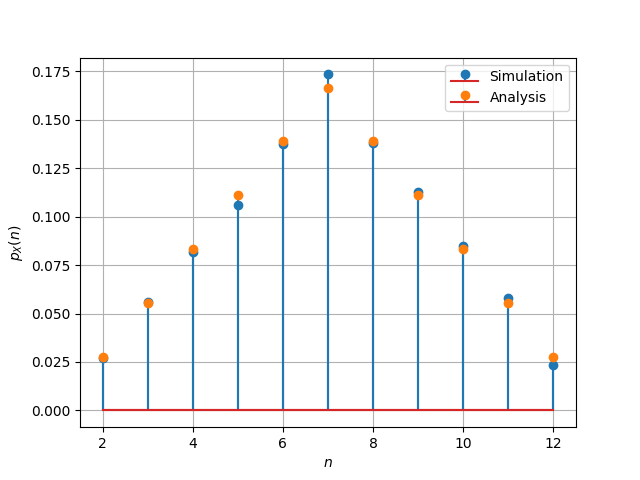
\includegraphics[width=\columnwidth]{./figs/sum/pmf.png}
\caption{Plot of $p_X(n)$.  Simulations are close to the analysis. }
\label{fig:dice}
\end{figure}
\item The python code is available in 
\begin{lstlisting}
/codes/sum/dice.py
\end{lstlisting}

%\item 
%We have shown how a simple problem of throwing a dice can be used for learning not just probability but concepts in  signal processing as well.  Inversion of the $Z$-transform for finding the pmf using contour integration, though not discussed here, opens a window to complex analysis too.  Note that the solutions that are provided  can be easily understood using high school math like arithmetic and geometric sums.  Thus, school students can use a bit of college level math to obtain simpler solutions to their problems.  College students can be exposed to advanced mathematics through simple problems from high school texts.  In addition, both can learn how to verify theoretical results through computer simulations.

%\bibliographystyle{tMES}
%\bibliography{school}
%
%\end{document}
\end{enumerate}

\section{Cumulative Distribution Function}
\subsection{The Bernoulli Distribution}
%%%%%%%%%%%%%%%%%%%%%%%%%%%%%%%%%%%%%%%%%%%%%%%%%%%%%%%%%%%%%%%%%%%%%%
%%                                                                  %%
%%  This is the header of a LaTeX2e file exported from Gnumeric.    %%
%%                                                                  %%
%%  This file can be compiled as it stands or included in another   %%
%%  LaTeX document. The table is based on the longtable package so  %%
%%  the longtable options (headers, footers...) can be set in the   %%
%%  preamble section below (see PRAMBLE).                           %%
%%                                                                  %%
%%  To include the file in another, the following two lines must be %%
%%  in the including file:                                          %%
%%        \def\inputGnumericTable{}                                 %%
%%  at the beginning of the file and:                               %%
%%        \input{name-of-this-file.tex}                             %%
%%  where the table is to be placed. Note also that the including   %%
%%  file must use the following packages for the table to be        %%
%%  rendered correctly:                                             %%
%%    \usepackage[latin1]{inputenc}                                 %%
%%    \usepackage{color}                                            %%
%%    \usepackage{array}                                            %%
%%    \usepackage{longtable}                                        %%
%%    \usepackage{calc}                                             %%
%%    \usepackage{multirow}                                         %%
%%    \usepackage{hhline}                                           %%
%%    \usepackage{ifthen}                                           %%
%%  optionally (for landscape tables embedded in another document): %%
%%    \usepackage{lscape}                                           %%
%%                                                                  %%
%%%%%%%%%%%%%%%%%%%%%%%%%%%%%%%%%%%%%%%%%%%%%%%%%%%%%%%%%%%%%%%%%%%%%%



%%  This section checks if we are begin input into another file or  %%
%%  the file will be compiled alone. First use a macro taken from   %%
%%  the TeXbook ex 7.7 (suggestion of Han-Wen Nienhuys).            %%
\def\ifundefined#1{\expandafter\ifx\csname#1\endcsname\relax}


%%  Check for the \def token for inputed files. If it is not        %%
%%  defined, the file will be processed as a standalone and the     %%
%%  preamble will be used.                                          %%
\ifundefined{inputGnumericTable}

%%  We must be able to close or not the document at the end.        %%
	\def\gnumericTableEnd{\end{document}}


%%%%%%%%%%%%%%%%%%%%%%%%%%%%%%%%%%%%%%%%%%%%%%%%%%%%%%%%%%%%%%%%%%%%%%
%%                                                                  %%
%%  This is the PREAMBLE. Change these values to get the right      %%
%%  paper size and other niceties.                                  %%
%%                                                                  %%
%%%%%%%%%%%%%%%%%%%%%%%%%%%%%%%%%%%%%%%%%%%%%%%%%%%%%%%%%%%%%%%%%%%%%%

	\documentclass[12pt%
			  %,landscape%
                    ]{report}
       \usepackage[latin1]{inputenc}
       \usepackage{fullpage}
       \usepackage{color}
       \usepackage{array}
       \usepackage{longtable}
       \usepackage{calc}
       \usepackage{multirow}
       \usepackage{hhline}
       \usepackage{ifthen}

	\begin{document}


%%  End of the preamble for the standalone. The next section is for %%
%%  documents which are included into other LaTeX2e files.          %%
\else

%%  We are not a stand alone document. For a regular table, we will %%
%%  have no preamble and only define the closing to mean nothing.   %%
    \def\gnumericTableEnd{}

%%  If we want landscape mode in an embedded document, comment out  %%
%%  the line above and uncomment the two below. The table will      %%
%%  begin on a new page and run in landscape mode.                  %%
%       \def\gnumericTableEnd{\end{landscape}}
%       \begin{landscape}


%%  End of the else clause for this file being \input.              %%
\fi

%%%%%%%%%%%%%%%%%%%%%%%%%%%%%%%%%%%%%%%%%%%%%%%%%%%%%%%%%%%%%%%%%%%%%%
%%                                                                  %%
%%  The rest is the gnumeric table, except for the closing          %%
%%  statement. Changes below will alter the table's appearance.     %%
%%                                                                  %%
%%%%%%%%%%%%%%%%%%%%%%%%%%%%%%%%%%%%%%%%%%%%%%%%%%%%%%%%%%%%%%%%%%%%%%

\providecommand{\gnumericmathit}[1]{#1} 
%%  Uncomment the next line if you would like your numbers to be in %%
%%  italics if they are italizised in the gnumeric table.           %%
%\renewcommand{\gnumericmathit}[1]{\mathit{#1}}
\providecommand{\gnumericPB}[1]%
{\let\gnumericTemp=\\#1\let\\=\gnumericTemp\hspace{0pt}}
 \ifundefined{gnumericTableWidthDefined}
        \newlength{\gnumericTableWidth}
        \newlength{\gnumericTableWidthComplete}
        \newlength{\gnumericMultiRowLength}
        \global\def\gnumericTableWidthDefined{}
 \fi
%% The following setting protects this code from babel shorthands.  %%
 \ifthenelse{\isundefined{\languageshorthands}}{}{\languageshorthands{english}}
%%  The default table format retains the relative column widths of  %%
%%  gnumeric. They can easily be changed to c, r or l. In that case %%
%%  you may want to comment out the next line and uncomment the one %%
%%  thereafter                                                      %%
\providecommand\gnumbox{\makebox[0pt]}
%%\providecommand\gnumbox[1][]{\makebox}

%% to adjust positions in multirow situations                       %%
\setlength{\bigstrutjot}{\jot}
\setlength{\extrarowheight}{\doublerulesep}

%%  The \setlongtables command keeps column widths the same across  %%
%%  pages. Simply comment out next line for varying column widths.  %%
\setlongtables

\setlength\gnumericTableWidth{%
	41pt+%
	14pt+%
	47pt+%
0pt}
\def\gumericNumCols{3}
\setlength\gnumericTableWidthComplete{\gnumericTableWidth+%
         \tabcolsep*\gumericNumCols*2+\arrayrulewidth*\gumericNumCols}
\ifthenelse{\lengthtest{\gnumericTableWidthComplete > \linewidth}}%
         {\def\gnumericScale{1*\ratio{\linewidth-%
                        \tabcolsep*\gumericNumCols*2-%
                        \arrayrulewidth*\gumericNumCols}%
{\gnumericTableWidth}}}%
{\def\gnumericScale{1}}

%%%%%%%%%%%%%%%%%%%%%%%%%%%%%%%%%%%%%%%%%%%%%%%%%%%%%%%%%%%%%%%%%%%%%%
%%                                                                  %%
%% The following are the widths of the various columns. We are      %%
%% defining them here because then they are easier to change.       %%
%% Depending on the cell formats we may use them more than once.    %%
%%                                                                  %%
%%%%%%%%%%%%%%%%%%%%%%%%%%%%%%%%%%%%%%%%%%%%%%%%%%%%%%%%%%%%%%%%%%%%%%

\ifthenelse{\isundefined{\gnumericColA}}{\newlength{\gnumericColA}}{}\settowidth{\gnumericColA}{\begin{tabular}{@{}p{41pt*\gnumericScale}@{}}x\end{tabular}}
\ifthenelse{\isundefined{\gnumericColB}}{\newlength{\gnumericColB}}{}\settowidth{\gnumericColB}{\begin{tabular}{@{}p{14pt*\gnumericScale}@{}}x\end{tabular}}
\ifthenelse{\isundefined{\gnumericColC}}{\newlength{\gnumericColC}}{}\settowidth{\gnumericColC}{\begin{tabular}{@{}p{47pt*\gnumericScale}@{}}x\end{tabular}}

\begin{tabular}[c]{%
	b{\gnumericColA}%
	b{\gnumericColB}%
	b{\gnumericColC}%
	}

%%%%%%%%%%%%%%%%%%%%%%%%%%%%%%%%%%%%%%%%%%%%%%%%%%%%%%%%%%%%%%%%%%%%%%
%%  The tabular options. (Caption, headers... see Goosens, p.124) %%
%	\caption{The Table Caption.}             \\	%
% \hline	% Across the top of the table.
%%  The rest of these options are table rows which are placed on    %%
%%  the first, last or every page. Use \multicolumn if you want.    %%

%%  Header for the first page.                                      %%
%	\multicolumn{3}{c}{The First Header} \\ \hline 
%	\multicolumn{1}{c}{colTag}	%Column 1
%	&\multicolumn{1}{c}{colTag}	%Column 2
%	&\multicolumn{1}{c}{colTag}	\\ \hline %Last column
%	\endfirsthead

%%  The running header definition.                                  %%
%	\hline
%	\multicolumn{3}{l}{\ldots\small\slshape continued} \\ \hline
%	\multicolumn{1}{c}{colTag}	%Column 1
%	&\multicolumn{1}{c}{colTag}	%Column 2
%	&\multicolumn{1}{c}{colTag}	\\ \hline %Last column
%	\endhead

%%  The running footer definition.                                  %%
%	\hline
%	\multicolumn{3}{r}{\small\slshape continued\ldots} \\
%	\endfoot

%%  The ending footer definition.                                   %%
%	\multicolumn{3}{c}{That's all folks} \\ \hline 
%	\endlastfoot
%%%%%%%%%%%%%%%%%%%%%%%%%%%%%%%%%%%%%%%%%%%%%%%%%%%%%%%%%%%%%%%%%%%%%%

\hhline{|-|-|-}
	 \multicolumn{1}{|p{\gnumericColA}|}%
	{\gnumericPB{\centering}\gnumbox{\textbf{Colour}}}
	&\multicolumn{1}{p{\gnumericColB}|}%
	{\gnumericPB{\centering}\gnumbox{\textbf{X}}}
	&\multicolumn{1}{p{\gnumericColC}|}%
	{\gnumericPB{\raggedright}\gnumbox[l]{\textbf{Number}}}
\\
\hhline{|---|}
	 \multicolumn{1}{|p{\gnumericColA}|}%
	{\gnumericPB{\centering}\gnumbox{Blue}}
	&\multicolumn{1}{p{\gnumericColB}|}%
	{\gnumericPB{\centering}\gnumbox{0}}
	&\multicolumn{1}{p{\gnumericColC}|}%
	{\gnumericPB{\raggedright}\gnumbox[l]{$n(X = 0)$}}
\\
\hhline{|---|}
	 \multicolumn{1}{|p{\gnumericColA}|}%
	{\gnumericPB{\centering}\gnumbox{Green}}
	&\multicolumn{1}{p{\gnumericColB}|}%
	{\gnumericPB{\centering}\gnumbox{1}}
	&\multicolumn{1}{p{\gnumericColC}|}%
	{\gnumericPB{\raggedright}\gnumbox[l]{$n(X = 1)$}}
\\
\hhline{|-|-|-|}
\end{tabular}

\ifthenelse{\isundefined{\languageshorthands}}{}{\languageshorthands{\languagename}}
\gnumericTableEnd

\subsection{The Binomial Distribution}
In a hurdle race, a player has to cross 10 hurdles. The probability that he will
clear each hurdle is $\frac{5}{6}$. What is the probability that he will knock down fewer than 2 hurdles?
\renewcommand{\theequation}{\theenumi}
\renewcommand{\thefigure}{\theenumi}
\begin{enumerate}[label=\thesubsection.\arabic*.,ref=\thesubsection.\theenumi]
\numberwithin{equation}{enumi}
\numberwithin{figure}{enumi}
\numberwithin{table}{enumi}
%
%
\item  Let $X_i \in \cbrak{0,1}$ represent the $ith$ hurdle where $1$ denotes a hurdle being knocked down.  Then, $X_i$ has a bernoulli distribution with parameter
\begin{align}
p = 1-\frac{5}{6} = \frac{1}{6}
\label{eq:p_binom_exam}
\end{align}

\item {\em The Binomial Distribution: } Let
\begin{align}
\label{eq:bern_binom}
X = \sum_{i=1}^{n}X_i
\end{align}
%
where $n$ is the total number of hurdles.
Then $X$ has a binomial distribution.  Then, for 
\begin{align}
p_{X_i}(n) \ztrans P_{X_i}(z),
\end{align}
yielding
\begin{align}
 P_{X_i}(z) = 1-p + pz^{-1}
\end{align}
 with
%
Using the fact that $X_i$ are i.i.d.,
\begin{align}
\label{eq:ztrans_binom}
 P_{X}(z) &= \brak{1-p + pz^{-1}}^n
\\
&= \sum_{k=0}^{n}\comb{n}{k}p^{k}\brak{1-p}^{n-k}z^{-k}
\\
\implies p_{X}(k) &= 
\begin{cases}
\comb{n}{k}p^{n-k}\brak{1-p}^k & 0 \le k \le n
\\
0 & \text{otherwise}
\end{cases}
\label{eq:pdf_binom}
\end{align}
%
The cumulative distribution function of $X$ is defined as
\begin{align}
F_{X}(r) = \pr{X\le r} = \sum_{k=0}^{r}\comb{n}{k}p^{k}\brak{1-p}^{n-k}
\label{eq:cdf_binom}
\end{align}
%
upon substituting from \eqref{eq:pdf_binom}.

\item {\em Evaluationg the Probability: }Substituting from \eqref{eq:p_binom_exam} in \eqref{eq:cdf_binom},

\begin {align}
\pr{X < 2} &= F_{X}(1)
\\
&=\sum_{k=0}^{1}\comb{n}{k}\brak{\frac{5}{6}}^{10-k}\brak{\frac{1}{6}}^k
\\
&=3\brak{\frac{5}{6}}^{10} = 0.4845167486695371 
\label{eq:bern_binom_ans}
\end{align}
%
which is the desired probability.
%
\item The following code verifies the above result.
\begin{lstlisting}
codes/binomial/binomial.py
\end{lstlisting}
\end{enumerate}

\section{Central Limit Theorem: Gaussian Distribution}
\renewcommand{\thefigure}{\theenumi}
\renewcommand{\thetable}{\theenumi}
%%
%\begin{enumerate}[label=\thesection.\arabic*
%,ref=\thesection.\theenumi]

\subsection{Bernoulli to Gaussian}
\begin{enumerate}[label=\thesubsection.\arabic*
,ref=\thesection.\theenumi]


\item {\em Mean :}  The mean of the bernoulli distribution is 
\begin{align}
\mu = E\brak{X_i}  = \sum_{k=0}^{1}kp_{X_i}(k) = p = \frac{1}{6}
\end{align}
\item {\em Moment:}  The moment of the distribution is defined as
\begin{align}
E\brak{X_i^r}  = \sum_{k=0}^{1}k^rp_{X_i}(k) = p = \frac{1}{6}
\end{align}

%The second moment of the bernoulli distribution is 
%\begin{align}
%E\brak{X_i}  = \sum_{k=0}^{1}kp_{X_i}(k) = p = \frac{1}{6}
%\end{align}
\item {\em Variance :}  The variance of the bernoulli distribution is defined as
\begin{align}
\sigma^2 &= E\brak{X-E\brak{X}}^2  = E\brak{X^2}-E^2\brak{X} 
\\
&=p-p^2 = p\brak{1-p} = \frac{5}{36}
\end{align}
%
The standard deviation 
\begin{align}
\sigma =  \sqrt{p\brak{1-p}}
\end{align}
%
\item {\em The Gaussian Distribution: }  Define
\begin{align}
\label{eq:bern_gauss}
G = \frac{1}{\sqrt{n}}\sum_{k=1}^{n}\frac{X_i-\mu}{\sigma}
\end{align}
%
\item {\em Approximating Binomial Using Gaussian: } From \eqref{eq:bern_gauss}
and \eqref{eq:bern_binom},
%
\begin{align}
X & \approx \sigma\sqrt{n}G + n\mu 
\\
\implies F_X(k) &= \pr{\sigma\sqrt{n}G + n\mu  \le k }
\\
 &= F_G\brak{\frac{k-n\mu}{\sigma\sqrt{n}}} \approx \phi\brak{\frac{k-n\mu}{\sigma\sqrt{n}}} 
\label{eq:bern_gaussian_cdf}
\end{align}
where 
\begin{align}
\phi_{X}(x) = \int^{x}_{-\infty} \frac{1}{\sqrt{2\pi}}e^{-\frac{x^2}{2}}, -\infty < x < \infty
\end{align}
\item The 
probability density function (PDF) 
of $G$ is
%
\begin{align}
p_{G}(x) &= \frac{d}{dx}F_{X}(x)
\\
 &=  \frac{1}{{\sigma\sqrt{n}}}\phi^{\prime}\brak{\frac{k-n\mu}{\sigma\sqrt{n}}} 
\label{eq:bern_gaussian_pdf}
\end{align}
%
For large $n$, $G$ is a continuous distribution with probability density function (PDF)
\begin{align}
p_G(x) =  \frac{1}{\sqrt{2\pi}}\exp\brak{-\frac{x^2}{2}}, -\infty < x < \infty,
\end{align}
%
\item {\em Evaluationg the Probability: }  From \ref{eq:bern_gaussian_cdf}
and \ref{eq:bern_gaussian_pdf},
\begin{align}
\pr{X \le 1 } &= F_{G}(1) = p_G(0)+p_G(1) 
\\
&\approx 
0.41299463887797094
\label{eq:bern_gauss_ans}
\end{align}
which is close to \eqref{eq:bern_binom_ans}.
%
\end{enumerate}
\subsection{Uniform to Gaussian}
\begin{enumerate}[label=\thesubsection.\arabic*
,ref=\thesection.\theenumi]

\item
Generate $10^6$ samples of the random variable
%
\begin{equation}
X = \sum_{i=1}^{12}U_i -6
\end{equation}
%
using a C program, where $U_i, i = 1,2,\dots, 12$ are  a set of independent uniform random variables between 0 and 1
and save in a file called gau.dat
\\
\solution Download the following files and execute the  C program.
\begin{lstlisting}
codes/cdf/exrand.c
codes/cdf/coeffs.h
\end{lstlisting}

%
\item
Load gau.dat in python and plot the empirical CDF of $X$ using the samples in gau.dat. What properties does a CDF have?
\\
\solution The CDF of $X$ is plotted in Fig. \ref{fig:gauss_cdf}
\begin{figure}
\centering
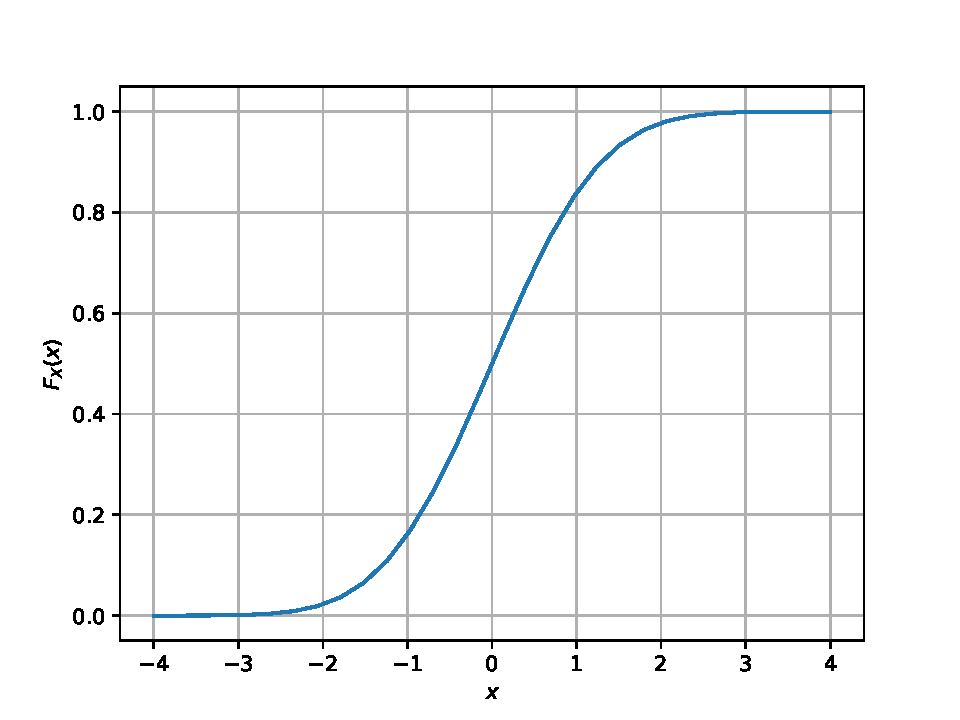
\includegraphics[width=\columnwidth]{./figs/clt/gauss_cdf}
\caption{The CDF of $X$}
\label{fig:gauss_cdf}
\end{figure}


\item
Load gau.dat in python and plot the empirical PDF of $X$ using the samples in gau.dat. The PDF of $X$ is defined as
\begin{align}
p_{X}(x) = \frac{d}{dx}F_{X}(x)
\end{align}
What properties does the PDF have?
\\
\solution The PDF of $X$ is plotted in Fig. \ref{fig:gauss_pdf} using the code below
\begin{lstlisting}
codes/clt/pdf_plot.py
\end{lstlisting}

\begin{figure}
\centering
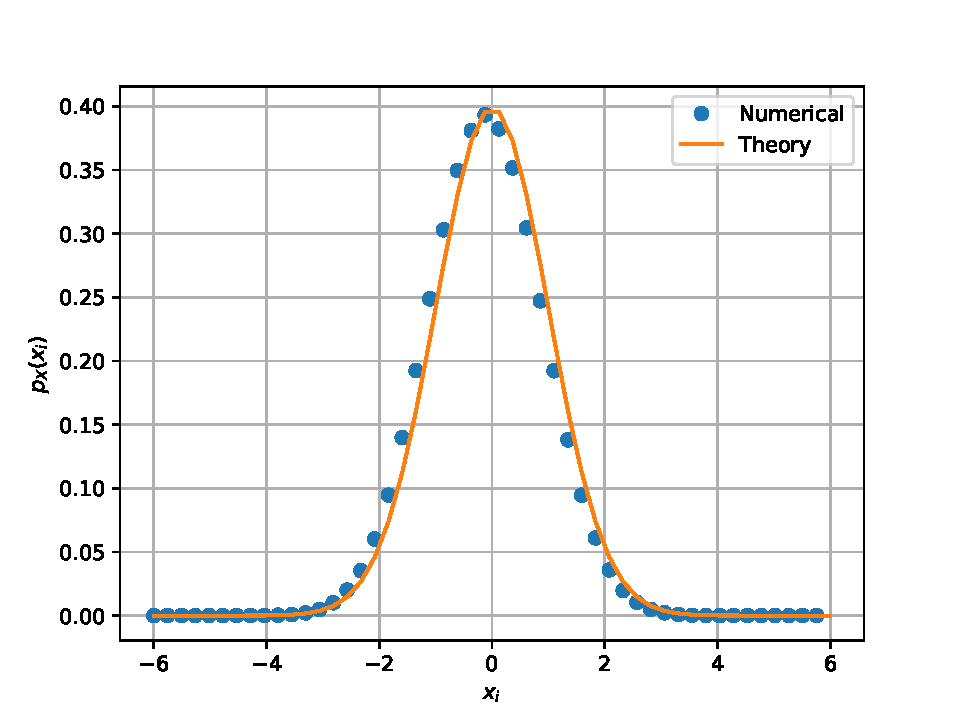
\includegraphics[width=\columnwidth]{./figs/clt/gauss_pdf}
\caption{The PDF of $X$}
\label{fig:gauss_pdf}
\end{figure}

\item Find the mean and variance of $X$ by writing a C program.
\\
\solution  Execute
\begin{lstlisting}
codes/clt/gaussian_numbers.c
\end{lstlisting}
\item Given that 
\begin{align}
p_{X}(x) = \frac{1}{\sqrt{2\pi}}\exp\brak{-\frac{x^2}{2}}, -\infty < x < \infty,
\label{eq:probman_gauss_pdf}
\end{align}
repeat the above exercise theoretically.
%
\\
\solution
Consider orthogonal vectors $\vec{m_1}$ and $\vec{m_2}$ to the given normal vector $\vec{n}$. Let, $\vec{m}$ = $\myvec{a\\b\\c}$, then
\begin{align}
\vec{m^T}\vec{n} &= 0\\
\implies\myvec{a&b&c}\myvec{3\\2\\-6} &= 0\\
\implies3a+2b-6c &= 0
\end{align}
Let a=1 and b=0 we get,
\begin{align}
\vec{m_1} &= \myvec{1\\0\\\frac{1}{2}} \label{eq:solutions/4/45/1/eq:eq1}
\end{align}
Let a=0 and b=1 we get,
\begin{align}
\vec{m_2} &= \myvec{0\\1\\\frac{1}{3}} \label{eq:solutions/4/45/1/eq:eq2}
\end{align}
Solving the equation,
\begin{align}
\vec{M}\vec{x} &= \vec{b}\label{eq:solutions/4/45/1/eq:eq3}
\end{align}
Substituting \eqref{eq:solutions/4/45/1/eq:eq1} and \eqref{eq:solutions/4/45/1/eq:eq2} in \eqref{eq:solutions/4/45/1/eq:eq3},
\begin{align}
    \myvec{1&0\\0&1\\\frac{1}{2}&\frac{1}{3}}\vec{x} &= \myvec{-3\\2\\1}\label{eq:solutions/4/45/1/eq:eq4}
\end{align}
Solving \eqref{eq:solutions/4/45/1/eq:eq4} using Singular Value Decomposition on $\vec{M}$ as follows,
\begin{align}
\vec{M}=\vec{U}\vec{\Sigma}\vec{V}^T\label{eq:solutions/4/45/1/eq:eq5}
\end{align}
Where the columns of $\vec{V}$ are the eigen vectors of $\vec{M}^T\vec{M}$ ,the columns of $\vec{U}$ are the eigen vectors of $\vec{M}\vec{M}^T$ and $\vec{S}$ is diagonal matrix of singular value of eigenvalues of $\vec{M}^T\vec{M}$. We have,
\begin{align}
\vec{M}^T\vec{M}=\myvec{\frac{5}{4}&\frac{1}{6}\\\frac{1}{6}&\frac{10}{9}}\label{eq:solutions/4/45/1/eq:eq6}\\
\vec{M}\vec{M}^T=\myvec{1&0&\frac{1}{2}\\0&1&\frac{1}{3}\\\frac{1}{2}&\frac{1}{3}&\frac{13}{36}}
\end{align}
Substituting \eqref{eq:solutions/4/45/1/eq:eq5} in \eqref{eq:solutions/4/45/1/eq:eq3},
\begin{align}
\vec{U}\vec{\Sigma}\vec{V}^T\vec{x} & = \vec{b}\\
\implies\vec{x} &= \vec{V}\vec{\Sigma^{-1}}\vec{U^T}\vec{b}\label{eq:solutions/4/45/1/eq:eq7}
\end{align}
Where $\vec{\Sigma^{-1}}$ is Moore-Penrose Pseudo-Inverse of $\vec{\Sigma}$ and is obtained by inversing only non-zero elements in $\vec{\Sigma}$\\
Calculating eigen values of $\vec{M}\vec{M}^T$,
\begin{align}
\mydet{\vec{M}\vec{M}^T - \lambda\vec{I}} &= 0\\
\implies\mydet{1-\lambda&0&\frac{1}{2}\\0&1-\lambda&\frac{1}{3}\\\frac{1}{2}&\frac{1}{3}&\frac{13}{36}-\lambda} &=0\\
\implies \lambda^3-\frac{85}{36}\lambda^2+\frac{49}{36}\lambda&=0 \label{eq:solutions/4/45/1/eq:eq8}
\end{align}
From the characteristic equation \eqref{eq:solutions/4/45/1/eq:eq8}, the eigen values of $\vec{M}\vec{M}^T$ are,
\begin{align}
\lambda_1 = \frac{49}{36} \quad
\lambda_2 = 1 \quad
\lambda_3 = 0
\end{align}
The eigen vectors of $\vec{M}\vec{M}^T$ are,
\begin{align}
\vec{u_1}=\myvec{\frac{18}{13}\\\frac{12}{13}\\1}\quad
\vec{u_2}=\myvec{\frac{-2}{3}\\1\\0}\quad
\vec{u_3}=\myvec{\frac{-1}{2}\\\frac{-1}{3}\\1}\label{eq:solutions/4/45/1/eq:eq9}
\end{align}
Normalizing the eigen vectors in equation \eqref{eq:solutions/4/45/1/eq:eq9}
\begin{align}
\vec{u_1}=\myvec{\frac{18}{7\sqrt{13}}\\\frac{12}{7\sqrt{13}}\\\frac{\sqrt{13}}{7}}\quad
\vec{u_2}=\myvec{\frac{-2}{\sqrt{13}}\\\frac{3}{\sqrt{13}}\\0}\quad
\vec{u_3}=\myvec{\frac{-7}{12}\\\frac{-7}{18}\\\frac{7}{6}}
\end{align}
Hence we obtain $\vec{U}$ as follows,
\begin{align}
\vec{U}=\myvec{\frac{18}{7\sqrt{13}}&\frac{-2}{\sqrt{13}}&\frac{-7}{12}\\\frac{12}{7\sqrt{13}}&\frac{3}{\sqrt{13}}&\frac{-7}{18}\\\frac{\sqrt{13}}{7}&0&\frac{7}{6}}\label{eq:solutions/4/45/1/eq:eq10}
\end{align}
By computing the singular values from eigen values $\lambda_1, \lambda_2, \lambda_3$ we get $\vec{\Sigma}$ as,
\begin{align}
\vec{\Sigma}=\myvec{\frac{49}{36}&0\\0&1\\0&0}
\end{align}
Calculating eigen values of $\vec{M}^T\vec{M}$,
\begin{align}
\mydet{\vec{M}^T\vec{M} - \lambda\vec{I}} &= 0\\
\implies\mydet{\frac{5}{4}-\lambda&\frac{1}{6}\\\frac{1}{6}&\frac{10}{9}-\lambda} &=0\\
\implies\lambda^2-\frac{85}{36}\lambda+\frac{49}{36} &=0
\end{align}
From the characteristic equation, the eigen values of $\vec{M}^T\vec{M}$ are,
\begin{align}
\lambda_1 = \frac{49}{36}\quad
\lambda_2 = 1
\end{align}
Hence the eigen vectors of $\vec{M}^T\vec{M}$ are,
\begin{align}
\vec{v}_1=\myvec{\frac{3}{2}\\1} \quad
\vec{v}_2=\myvec{\frac{-2}{3}\\1}
\end{align}
Normalizing the eigen vectors,
\begin{align}
\vec{v}_1=\myvec{\frac{3}{\sqrt{13}}\\\frac{2}{\sqrt{13}}} \quad
\vec{v}_2=\myvec{\frac{-2}{\sqrt{13}}\\\frac{3}{\sqrt{13}}}
\end{align}
Hence we obtain $\vec{V}$ as,
\begin{align}
\vec{V}=\myvec{\frac{3}{\sqrt{13}}&\frac{-2}{\sqrt{13}}\\\frac{2}{\sqrt{13}}&\frac{3}{\sqrt{13}}}
\end{align}
From \eqref{eq:solutions/4/45/1/eq:eq3}, the Singular Value Decomposition of $\vec{M}$ is as follows,
\begin{align}
\vec{M} = \myvec{\frac{18}{7\sqrt{13}}&\frac{-2}{\sqrt{13}}&\frac{-7}{12}\\\frac{12}{7\sqrt{13}}&\frac{3}{\sqrt{13}}&\frac{-7}{18}\\\frac{\sqrt{13}}{7}&0&\frac{7}{6}}\myvec{\frac{49}{36}&0\\0&1\\0&0}\myvec{\frac{3}{\sqrt{13}}&\frac{-2}{\sqrt{13}}\\\frac{2}{\sqrt{13}}&\frac{3}{\sqrt{13}}}^T
\end{align}
And, the Moore-Penrose Pseudo inverse of $\vec{\Sigma}$ is given by,
\begin{align}
\vec{\Sigma^{-1}} = \myvec{\frac{6}{7}&0&0\\0&1&0}
\end{align}
From \eqref{eq:solutions/4/45/1/eq:eq7} we get,
\begin{align}
\vec{U}^T\vec{b}&=\myvec{\frac{-17}{7\sqrt{13}}\\\frac{12}{\sqrt{13}}\\\frac{77}{36}}\\
\vec{\Sigma^{-1}}\vec{U}^T\vec{b}&=\myvec{\frac{-102}{49\sqrt{13}}\\\frac{12}{\sqrt{13}}}\\
\vec{x} &= \vec{V}\vec{\Sigma^{-1}}\vec{U}^T\vec{b} &= \myvec{\frac{-114}{49}\\\frac{120}{49}}\label{eq:solutions/4/45/1/eq:eq11}
\end{align}
Now we verify the solution \eqref{eq:solutions/4/45/1/eq:eq11} using,
\begin{align}
\vec{M}\vec{x}=\vec{b}
\implies\vec{M}^T\vec{M}\vec{x} = \vec{M}^T\vec{b}\label{eq:solutions/4/45/1/eqVerify}
\end{align}
On evaluating the R.H.S in \eqref{eq:solutions/4/45/1/eqVerify} we get,
\begin{align}
\vec{M}^T\vec{M}\vec{x} &= \myvec{\frac{-5}{2}\\\frac{7}{3}}\\
\implies\myvec{\frac{5}{4}&\frac{1}{6}\\\frac{1}{6}&\frac{10}{9}}\vec{x} &= \myvec{\frac{-5}{2}\\\frac{7}{3}}\label{eq:solutions/4/45/1/eq:eq12}
\end{align}
On solving the augmented matrix of \eqref{eq:solutions/4/45/1/eq:eq12} we get,
\begin{align}
\myvec{\frac{5}{4}&\frac{1}{6}&\frac{-5}{2}\\\frac{1}{6}&\frac{10}{9}&\frac{7}{3}} &\xleftrightarrow{R_1=\frac{4R_1}{5}}\myvec{1&\frac{2}{15}&-2\\\frac{1}{6}&\frac{10}{9}&\frac{7}{3}}\\
&\xleftrightarrow{R_2=R_2-\frac{R_1}{6}}\myvec{1&\frac{2}{15}&-2\\0&\frac{49}{45}&\frac{8}{3}}\\
&\xleftrightarrow{R_2=\frac{45}{49}R_2}\myvec{1&\frac{2}{15}&-2\\0&1&\frac{120}{49}}\\
&\xleftrightarrow{R_1=R_1-\frac{2R_2}{15}}\myvec{1&0&\frac{-114}{49}\\0&1&\frac{120}{49}}\label{eq:solutions/4/45/1/eq:eq13}
\end{align}
From equation \eqref{eq:solutions/4/45/1/eq:eq13}, solution is given by,
\begin{align}
\vec{x}=\myvec{\frac{-114}{49}\\\frac{120}{49}}\label{eq:solutions/4/45/1/eq:eq14}
\end{align}
From the equations \eqref{eq:solutions/4/45/1/eq:eq11} and \eqref{eq:solutions/4/45/1/eq:eq14}, the solution $\vec{x}$ is verified.

\item Let $U$ be a uniform random variable between 0 and 1.
%\begin{enumerate}[label=\thesection.\arabic*
%,ref=\thesection.\theenumi]

%
\item
Load the uni.dat file into python and plot the empirical CDF of $U$ using the samples in uni.dat. The CDF is defined as
\begin{align}
F_{U}(x) = \pr{U \le x}
\end{align}
\\
\solution  The following code plots Fig. \ref{fig:uni_cdf}
\begin{lstlisting}
codes/cdf/cdf_plot.py
\end{lstlisting}
\begin{figure}
\centering
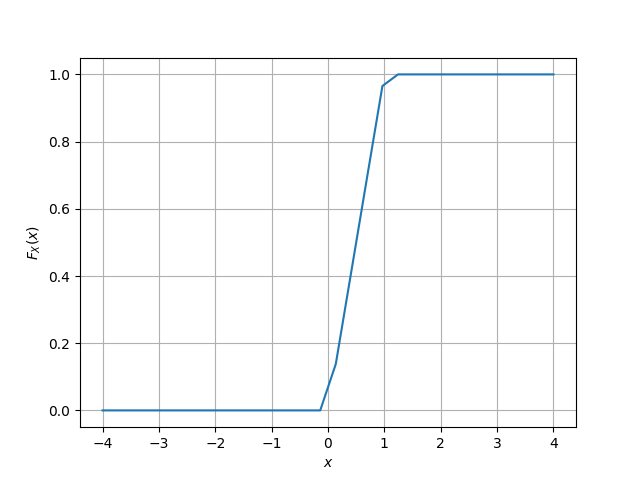
\includegraphics[width=\columnwidth]{./figs/cdf/uni_cdf}
\caption{The CDF of $U$}
\label{fig:uni_cdf}
\end{figure}

%\item Generate $10^6$ samples of $U$ using a C program and save into a file called uni.dat .
%\\


%
\item
Find a  theoretical expression for $F_{U}(x)$.

\item
The mean of $U$ is defined as
%
\begin{equation}
E\sbrak{U} = \frac{1}{N}\sum_{i=1}^{N}U_i
\end{equation}
%
and its variance as
%
\begin{equation}
\text{var}\sbrak{U} = E\sbrak{U- E\sbrak{U}}^2 
\end{equation}

Write a C program to  find the mean and variance of $U$. 
\item Verify your result theoretically given that
%
\begin{equation}
E\sbrak{U^k} = \int_{-\infty}^{\infty}x^kdF_{U}(x)
\end{equation}

\end{enumerate}




%\section{Cumulative Distribution Function}
%\renewcommand{\thefigure}{\theenumi}
\renewcommand{\thetable}{\theenumi}
%%
Let $U$ be a uniform random variable between 0 and 1.
%\begin{enumerate}[label=\thesection.\arabic*
%,ref=\thesection.\theenumi]
\item Generate $10^6$ samples of $U$ using a C program and save into a file called uni.dat .
\\
\solution Download the following files and execute the  C program.
\begin{lstlisting}
codes/cdf/exrand.c
codes/cdf/coeffs.h
\end{lstlisting}

%
\item
Load the uni.dat file into python and plot the empirical CDF of $U$ using the samples in uni.dat. The CDF is defined as
\begin{align}
F_{U}(x) = \pr{U \le x}
\end{align}
\\
\solution  The following code plots Fig. \ref{fig:uni_cdf}
\begin{lstlisting}
codes/cdf/cdf_plot.py
\end{lstlisting}
\begin{figure}
\centering
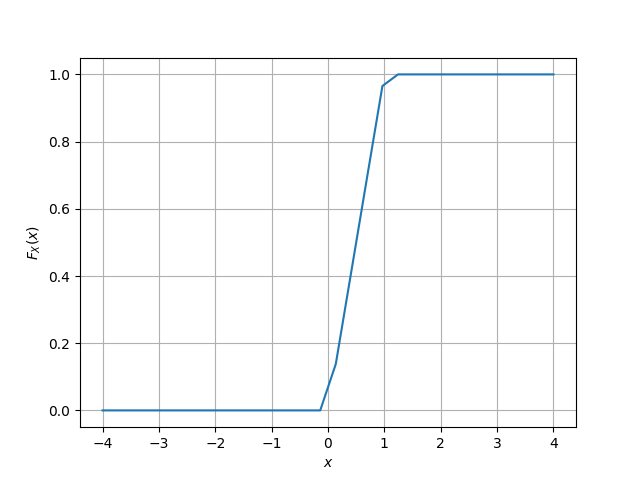
\includegraphics[width=\columnwidth]{./figs/cdf/uni_cdf}
\caption{The CDF of $U$}
\label{fig:uni_cdf}
\end{figure}

%
\item
Find a  theoretical expression for $F_{U}(x)$.

\item
The mean of $U$ is defined as
%
\begin{equation}
E\sbrak{U} = \frac{1}{N}\sum_{i=1}^{N}U_i
\end{equation}
%
and its variance as
%
\begin{equation}
\text{var}\sbrak{U} = E\sbrak{U- E\sbrak{U}}^2 
\end{equation}

Write a C program to  find the mean and variance of $U$. 
\item Verify your result theoretically given that
%
\begin{equation}
E\sbrak{U^k} = \int_{-\infty}^{\infty}x^kdF_{U}(x)
\end{equation}
%
\end{enumerate}





%\section{Bernoulli Distribution}
%\subsection{Distance from a plane to a point}
%%%%%%%%%%%%%%%%%%%%%%%%%%%%%%%%%%%%%%%%%%%%%%%%%%%%%%%%%%%%%%%%%%%%%%%
%%                                                                  %%
%%  This is the header of a LaTeX2e file exported from Gnumeric.    %%
%%                                                                  %%
%%  This file can be compiled as it stands or included in another   %%
%%  LaTeX document. The table is based on the longtable package so  %%
%%  the longtable options (headers, footers...) can be set in the   %%
%%  preamble section below (see PRAMBLE).                           %%
%%                                                                  %%
%%  To include the file in another, the following two lines must be %%
%%  in the including file:                                          %%
%%        \def\inputGnumericTable{}                                 %%
%%  at the beginning of the file and:                               %%
%%        \input{name-of-this-file.tex}                             %%
%%  where the table is to be placed. Note also that the including   %%
%%  file must use the following packages for the table to be        %%
%%  rendered correctly:                                             %%
%%    \usepackage[latin1]{inputenc}                                 %%
%%    \usepackage{color}                                            %%
%%    \usepackage{array}                                            %%
%%    \usepackage{longtable}                                        %%
%%    \usepackage{calc}                                             %%
%%    \usepackage{multirow}                                         %%
%%    \usepackage{hhline}                                           %%
%%    \usepackage{ifthen}                                           %%
%%  optionally (for landscape tables embedded in another document): %%
%%    \usepackage{lscape}                                           %%
%%                                                                  %%
%%%%%%%%%%%%%%%%%%%%%%%%%%%%%%%%%%%%%%%%%%%%%%%%%%%%%%%%%%%%%%%%%%%%%%



%%  This section checks if we are begin input into another file or  %%
%%  the file will be compiled alone. First use a macro taken from   %%
%%  the TeXbook ex 7.7 (suggestion of Han-Wen Nienhuys).            %%
\def\ifundefined#1{\expandafter\ifx\csname#1\endcsname\relax}


%%  Check for the \def token for inputed files. If it is not        %%
%%  defined, the file will be processed as a standalone and the     %%
%%  preamble will be used.                                          %%
\ifundefined{inputGnumericTable}

%%  We must be able to close or not the document at the end.        %%
	\def\gnumericTableEnd{\end{document}}


%%%%%%%%%%%%%%%%%%%%%%%%%%%%%%%%%%%%%%%%%%%%%%%%%%%%%%%%%%%%%%%%%%%%%%
%%                                                                  %%
%%  This is the PREAMBLE. Change these values to get the right      %%
%%  paper size and other niceties.                                  %%
%%                                                                  %%
%%%%%%%%%%%%%%%%%%%%%%%%%%%%%%%%%%%%%%%%%%%%%%%%%%%%%%%%%%%%%%%%%%%%%%

	\documentclass[12pt%
			  %,landscape%
                    ]{report}
       \usepackage[latin1]{inputenc}
       \usepackage{fullpage}
       \usepackage{color}
       \usepackage{array}
       \usepackage{longtable}
       \usepackage{calc}
       \usepackage{multirow}
       \usepackage{hhline}
       \usepackage{ifthen}

	\begin{document}


%%  End of the preamble for the standalone. The next section is for %%
%%  documents which are included into other LaTeX2e files.          %%
\else

%%  We are not a stand alone document. For a regular table, we will %%
%%  have no preamble and only define the closing to mean nothing.   %%
    \def\gnumericTableEnd{}

%%  If we want landscape mode in an embedded document, comment out  %%
%%  the line above and uncomment the two below. The table will      %%
%%  begin on a new page and run in landscape mode.                  %%
%       \def\gnumericTableEnd{\end{landscape}}
%       \begin{landscape}


%%  End of the else clause for this file being \input.              %%
\fi

%%%%%%%%%%%%%%%%%%%%%%%%%%%%%%%%%%%%%%%%%%%%%%%%%%%%%%%%%%%%%%%%%%%%%%
%%                                                                  %%
%%  The rest is the gnumeric table, except for the closing          %%
%%  statement. Changes below will alter the table's appearance.     %%
%%                                                                  %%
%%%%%%%%%%%%%%%%%%%%%%%%%%%%%%%%%%%%%%%%%%%%%%%%%%%%%%%%%%%%%%%%%%%%%%

\providecommand{\gnumericmathit}[1]{#1} 
%%  Uncomment the next line if you would like your numbers to be in %%
%%  italics if they are italizised in the gnumeric table.           %%
%\renewcommand{\gnumericmathit}[1]{\mathit{#1}}
\providecommand{\gnumericPB}[1]%
{\let\gnumericTemp=\\#1\let\\=\gnumericTemp\hspace{0pt}}
 \ifundefined{gnumericTableWidthDefined}
        \newlength{\gnumericTableWidth}
        \newlength{\gnumericTableWidthComplete}
        \newlength{\gnumericMultiRowLength}
        \global\def\gnumericTableWidthDefined{}
 \fi
%% The following setting protects this code from babel shorthands.  %%
 \ifthenelse{\isundefined{\languageshorthands}}{}{\languageshorthands{english}}
%%  The default table format retains the relative column widths of  %%
%%  gnumeric. They can easily be changed to c, r or l. In that case %%
%%  you may want to comment out the next line and uncomment the one %%
%%  thereafter                                                      %%
\providecommand\gnumbox{\makebox[0pt]}
%%\providecommand\gnumbox[1][]{\makebox}

%% to adjust positions in multirow situations                       %%
\setlength{\bigstrutjot}{\jot}
\setlength{\extrarowheight}{\doublerulesep}

%%  The \setlongtables command keeps column widths the same across  %%
%%  pages. Simply comment out next line for varying column widths.  %%
\setlongtables

\setlength\gnumericTableWidth{%
	41pt+%
	14pt+%
	47pt+%
0pt}
\def\gumericNumCols{3}
\setlength\gnumericTableWidthComplete{\gnumericTableWidth+%
         \tabcolsep*\gumericNumCols*2+\arrayrulewidth*\gumericNumCols}
\ifthenelse{\lengthtest{\gnumericTableWidthComplete > \linewidth}}%
         {\def\gnumericScale{1*\ratio{\linewidth-%
                        \tabcolsep*\gumericNumCols*2-%
                        \arrayrulewidth*\gumericNumCols}%
{\gnumericTableWidth}}}%
{\def\gnumericScale{1}}

%%%%%%%%%%%%%%%%%%%%%%%%%%%%%%%%%%%%%%%%%%%%%%%%%%%%%%%%%%%%%%%%%%%%%%
%%                                                                  %%
%% The following are the widths of the various columns. We are      %%
%% defining them here because then they are easier to change.       %%
%% Depending on the cell formats we may use them more than once.    %%
%%                                                                  %%
%%%%%%%%%%%%%%%%%%%%%%%%%%%%%%%%%%%%%%%%%%%%%%%%%%%%%%%%%%%%%%%%%%%%%%

\ifthenelse{\isundefined{\gnumericColA}}{\newlength{\gnumericColA}}{}\settowidth{\gnumericColA}{\begin{tabular}{@{}p{41pt*\gnumericScale}@{}}x\end{tabular}}
\ifthenelse{\isundefined{\gnumericColB}}{\newlength{\gnumericColB}}{}\settowidth{\gnumericColB}{\begin{tabular}{@{}p{14pt*\gnumericScale}@{}}x\end{tabular}}
\ifthenelse{\isundefined{\gnumericColC}}{\newlength{\gnumericColC}}{}\settowidth{\gnumericColC}{\begin{tabular}{@{}p{47pt*\gnumericScale}@{}}x\end{tabular}}

\begin{tabular}[c]{%
	b{\gnumericColA}%
	b{\gnumericColB}%
	b{\gnumericColC}%
	}

%%%%%%%%%%%%%%%%%%%%%%%%%%%%%%%%%%%%%%%%%%%%%%%%%%%%%%%%%%%%%%%%%%%%%%
%%  The tabular options. (Caption, headers... see Goosens, p.124) %%
%	\caption{The Table Caption.}             \\	%
% \hline	% Across the top of the table.
%%  The rest of these options are table rows which are placed on    %%
%%  the first, last or every page. Use \multicolumn if you want.    %%

%%  Header for the first page.                                      %%
%	\multicolumn{3}{c}{The First Header} \\ \hline 
%	\multicolumn{1}{c}{colTag}	%Column 1
%	&\multicolumn{1}{c}{colTag}	%Column 2
%	&\multicolumn{1}{c}{colTag}	\\ \hline %Last column
%	\endfirsthead

%%  The running header definition.                                  %%
%	\hline
%	\multicolumn{3}{l}{\ldots\small\slshape continued} \\ \hline
%	\multicolumn{1}{c}{colTag}	%Column 1
%	&\multicolumn{1}{c}{colTag}	%Column 2
%	&\multicolumn{1}{c}{colTag}	\\ \hline %Last column
%	\endhead

%%  The running footer definition.                                  %%
%	\hline
%	\multicolumn{3}{r}{\small\slshape continued\ldots} \\
%	\endfoot

%%  The ending footer definition.                                   %%
%	\multicolumn{3}{c}{That's all folks} \\ \hline 
%	\endlastfoot
%%%%%%%%%%%%%%%%%%%%%%%%%%%%%%%%%%%%%%%%%%%%%%%%%%%%%%%%%%%%%%%%%%%%%%

\hhline{|-|-|-}
	 \multicolumn{1}{|p{\gnumericColA}|}%
	{\gnumericPB{\centering}\gnumbox{\textbf{Colour}}}
	&\multicolumn{1}{p{\gnumericColB}|}%
	{\gnumericPB{\centering}\gnumbox{\textbf{X}}}
	&\multicolumn{1}{p{\gnumericColC}|}%
	{\gnumericPB{\raggedright}\gnumbox[l]{\textbf{Number}}}
\\
\hhline{|---|}
	 \multicolumn{1}{|p{\gnumericColA}|}%
	{\gnumericPB{\centering}\gnumbox{Blue}}
	&\multicolumn{1}{p{\gnumericColB}|}%
	{\gnumericPB{\centering}\gnumbox{0}}
	&\multicolumn{1}{p{\gnumericColC}|}%
	{\gnumericPB{\raggedright}\gnumbox[l]{$n(X = 0)$}}
\\
\hhline{|---|}
	 \multicolumn{1}{|p{\gnumericColA}|}%
	{\gnumericPB{\centering}\gnumbox{Green}}
	&\multicolumn{1}{p{\gnumericColB}|}%
	{\gnumericPB{\centering}\gnumbox{1}}
	&\multicolumn{1}{p{\gnumericColC}|}%
	{\gnumericPB{\raggedright}\gnumbox[l]{$n(X = 1)$}}
\\
\hhline{|-|-|-|}
\end{tabular}

\ifthenelse{\isundefined{\languageshorthands}}{}{\languageshorthands{\languagename}}
\gnumericTableEnd

\section{Stochastic Geometry}
Suppose you drop a die at random on the rectangular region shown in Fig. \ref{fig:chapters/uniform/1/}. What is the probability that it will land inside the circle with diameter 1m?
\renewcommand{\theequation}{\theenumi}
\renewcommand{\thefigure}{\theenumi}
\begin{enumerate}[label=\thesection.\arabic*.,ref=\thesection.\theenumi]
\numberwithin{equation}{enumi}
\numberwithin{figure}{enumi}
%
\item 
\begin{figure}[!ht]
\centering
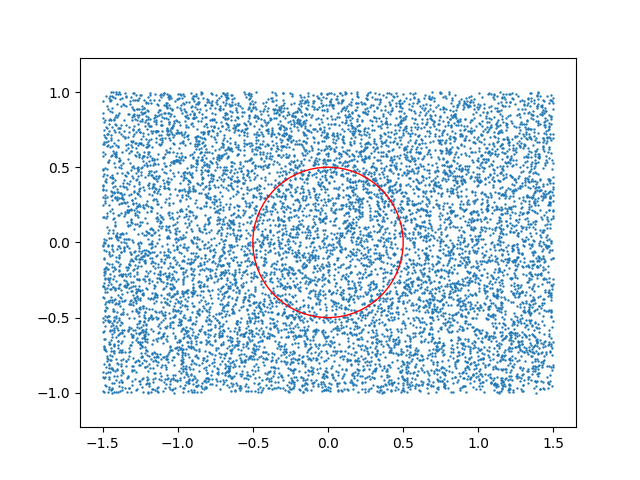
\includegraphics[width=\columnwidth]{./figs/stochastic/rectangle.png}
\caption{}
\label{fig:chapters/uniform/1/}
\end{figure}
%\\
%\solution
In Fig. \ref{fig:chapters/uniform/1/}, the sample size $S$ is the area of the rectangle given by 
\begin{align}
S=3\times 2=6 m^2
\end{align}
The event size is the area of the circle given by 
\begin{align}
E = \pi\brak{\frac{1}{2}}^2=\frac{\pi}{4} m^2 
\end{align}
The probabilty of the dice landing in the circle is
\begin{align}
\pr{E} = \frac{E}{S} = \frac{\pi}{24}
\label{eq:chapters/uniform/1/prob}
\end{align}
%
\item The python code is available in 
\begin{lstlisting}
/codes/stochastic/rect.py
\end{lstlisting}
The python code generates 10,000 points uniformly within the rectangle of dimensions $3 \times 2$ and checks for the number of points within the circle of radius 0.5.  The ratio of these is close to $\frac{\pi}{24}$.  Note that each time the code is run, the ratio will change, but will still be close to $\frac{\pi}{24}$.



\end{enumerate}

\section{Transformation of Variables}
\renewcommand{\theequation}{\theenumi}
\renewcommand{\thefigure}{\theenumi}

%\subsection{Independence}
\subsection{Using Definition}
\begin{enumerate}[label=\thesubsection.\arabic*.,ref=\thesubsection.\theenumi]
\numberwithin{equation}{enumi}
\numberwithin{figure}{enumi}

%
\item
Let $X_1 \sim  \gauss{0}{1}$ and $X_2 \sim  \gauss{0}{1}$. Plot the CDF and PDF of
%
\begin{equation}
V = X_1^2 + X_2^2 
\end{equation}
%
% \solution The following code generates the simulated CDF in Fig. \ref{fig:probman_trans_cdf_V}
% %
% \begin{figure}[!ht]
% \centering
% 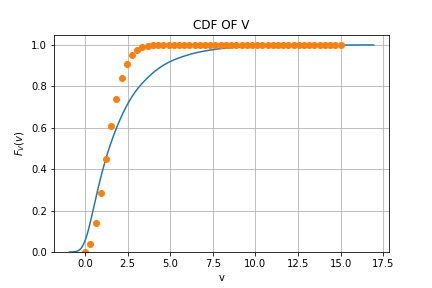
\includegraphics[width=\columnwidth]{figs/trans/cdf_V.png}
% \caption{CDF of $V$}
% \label{fig:probman_trans_cdf_V}
% \end{figure}
% %
% and the PDF in Fig. \ref{fig:probman_trans_pdf_V}
% %
% \begin{figure}[!ht]
% \centering
% 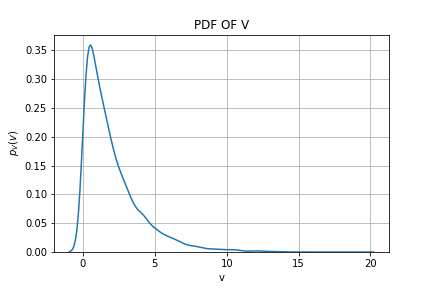
\includegraphics[width=\columnwidth]{figs/trans/pdf_V.png}
% \caption{PDF of $V$}
% \label{fig:probman_trans_pdf_V}
% \end{figure}
%

\item
If
%
\begin{equation}
F_{V}(x) = 
\begin{cases}
1 - e^{-\alpha x} & x \geq 0 \\
0 & x < 0,
\end{cases}
\label{eq:probman_F_V_alpha}
\end{equation}
%
find $\alpha$.

%
\item
\label{ch3_raleigh_sim}
Plot the CDF and PDf of
%
\begin{equation}
A = \sqrt{V}
\end{equation}
%

%
\item
Find an expression for $F_{A}(x)$ using the definition. Plot this expression and compare with the result of problem \ref{ch3_raleigh_sim}. 
\\
\solution 
% Given,
% \begin{align}
% A = \sqrt{V}
% \end{align}

\begin{align} 
F_A(x) &= \pr{A \le x} = \pr{\sqrt{V} \le x}
\\
&= \pr{V \le x^2} = F_V\brak{x^2}
\end{align}
%
From \eqref{eq:probman_F_V_alpha}, 
\begin{align} 
F_V\brak{x^2} = 
\begin{cases}
1 - e^{-\alpha x^2} & x \geq 0 \\
0 & x < 0,
\end{cases}
\end{align}
%
Substituting 

\begin{align}
\alpha = \frac{1}{2}
\end{align}

%
\begin{align} 
F_V\brak{x^2} = 
\begin{cases}
1 - e^{- \frac{x^2}{2}} & x \geq 0 \\
0 & x < 0,
\end{cases}
\end{align}
%
\item
Find an expression for $p_{A}(x)$.
\\
\solution
The PDf is obtained as
\begin{align}
f_V\brak{x^2} &= \frac{d}{dx}F_V\brak{x^2}
\\
&=
\begin{cases}
x e^{- \frac{x^2}{2}} & x \geq 0 \\
0 & x < 0,
\end{cases}
\end{align}
%
\end{enumerate}

%
\subsection{Using Jacobian}
%
\begin{enumerate}[label=\thesubsection.\arabic*.,ref=\thesubsection.\theenumi]
\numberwithin{equation}{enumi}
\numberwithin{figure}{enumi}

\item
Evaluate the joint PDF of $X_1,X_2$,  given by
%
\begin{equation}
p_{X_1,X_2}(x_1,x_2) = p_{X_1}\brak{x_1}p_{X_2}\brak{x_2}
\end{equation}
%
\solution From \eqref{eq:probman_gauss_pdf}
\begin{align}
p_{X_1}(x_1)&=\frac {1}{\sqrt {2\pi }}e^{-\frac {x_1^2}{2}}
\\
p_{X_2}(x_2)&=\frac {1}{\sqrt {2\pi }}e^{-\frac {x_2^2}{2}}
\\
\implies p_{X_1,X_2}(x_1,x_2) &= \frac {1}{\sqrt {2\pi }}e^{-\frac {x_1^2+x_2^2}{2}}
\label{eq:probman_pdf_x1x2}
\end{align}
 
%
\item
Let 
\begin{align}
 X_1 = \sqrt{V}\cos \theta
\\
 X_2 = \sqrt{V} \sin \theta.
\end{align}
Evaluate the Jacobian 
%
\begin{equation}
J =
\begin{vmatrix}
\frac{\partial x_1}{\partial v} & \frac{\partial x_2}{\partial v} \\
\frac{\partial x_1}{\partial \theta} & \frac{\partial x_2}{\partial \theta} 
\end{vmatrix}
\end{equation}
%
\solution
\begin{align}
J=\begin{vmatrix}
     \frac{1}{2\sqrt{v}}\cos\theta & \frac{1}{2\sqrt{v}}\sin\theta\\
       -v\sin\theta & v\cos\theta
\end{vmatrix}=\frac{1}{2}
\label{eq:probman_jacob_V}
\end{align}
\item
Find
%
\begin{equation}
p_{V,\Theta}\brak{v,\theta} = \abs{J}p_{X_1,X_2}\brak{x_1,x_2}
\end{equation}
%
\solution From \eqref{eq:probman_jacob_V} and \eqref{eq:probman_pdf_x1x2},
\begin{align}
p_{V,\Theta}\brak{v,\theta}=\frac{1}{4\pi}\exp{-\frac{v}{2}}, v \ge 0, 0 < \theta < 2\pi
\label{eq:probman_pdf_V_theta}
\end{align}
%
\item
Find $p_{V}(v)$.
\\
\solution For $v \ge 0$, from \eqref{eq:probman_pdf_V_theta},
\begin{align}
p_{V}(v) &= \int_{0}^{2\pi} \frac{1}{4\pi}\exp{-\frac{v}{2}} d \theta \\
&= \brak{2\pi} \times \frac{1}{4\pi}\exp{-\frac{v}{2}} \\
&= \frac{1}{2}\exp{-\frac{v}{2}}\\
\therefore p_{V}(v) &= 
\begin{cases}
\frac{1}{2}\exp{-\frac{v}{2}} & v\geq 0 \\
0 & v< 0
\end{cases}
\label{eq:probman_pdf_V}
\end{align}
%

\item
Find $p_{\Theta}(\theta)$.  
\\
\solution For $0 \le \theta \le 2\pi$, from \eqref{eq:probman_pdf_V_theta},
\begin{align}
p_{\Theta}(\theta) &= \int_{0}^{\infty} \frac{1}{4\pi}\exp{-\frac{v}{2}} d v \\
&= \frac{1}{2\pi} \left[1 - e^{-\frac{x}{2}} \right]_{0}^{\infty}\\
&= \frac{1}{2\pi}\\
\therefore p_{V}(v) &= 
\begin{cases}
\frac{1}{2\pi} & 0 \leq \theta \leq 2\pi \\
0 & \text{otherwise}
\end{cases}
\end{align}
%
\item
Are $V$ and $\Theta$ independent?
\\
\solution Yes,
\begin{align}
\because p_{V}(v)p_{\Theta}(\theta) &= \frac{1}{2}\exp{-\frac{v}{2}} \times \frac{1}{2\pi}\\
&= \frac{1}{4\pi}\exp{-\frac{v}{2}}\\
&= p_{V,\Theta}\brak{v,\theta}
\end{align}
\item
Find $p_{A}(x)$ using the Jacobian.
\\
\solution 
\begin{align}
p_{A}(x) &= \Pr(A=x) = \Pr(\sqrt{V} = x) \\
&= \Pr(V=x^2) = p_V(x^2)
\end{align}
From \eqref{eq:probman_pdf_V}, as $x^2 \ge 0$,
\begin{align}
p_{V}(x^2) &= \frac{1}{2}\exp{-\frac{x^2}{2}} 
\end{align}
%%
%\item
%Let $X_1 \sim  \gauss{2}{1}$ and $X_2 \sim  \gauss{3}{1}$. Find $E\sbrak{X_1X_2}$.  Try with different mean and variances. Comment.
%
%

%\section{The Transform Domain}
%\item
%Find the MGF of $X \sim \gauss{\mu}{\sigma^2}$. 
%
%\item
%Find the MGF of $Y$.
%
%%
%\item
%Find the PDF of $Y$ by inverting the MGF.
%
%%
\end{enumerate}

%
\section{Conditional Probability}
\begin{enumerate}[label=\thesection.\arabic*.,ref=\thesection.\theenumi]
\numberwithin{equation}{enumi}
\numberwithin{figure}{enumi}
%%
\item
\label{ch4_sim}
Plot 
\begin{equation}
P_e = \pr{\hat{X} = -1|X=1}
\end{equation}
%
for 
\begin{equation}
Y = AX+N,
\end{equation}
where $A$ is Raleigh with $E\sbrak{A^2} = \gamma, N \sim \gauss{0}{1}, X \in \brak{-1,1}$ for $0 \le \gamma \le 10$ dB.

%
\item
Assuming that $N$ is a constant, find an expression for $P_e$.  Call this $P_e(N)$

%
\item
%
\label{ch4_anal}
For a function $g$,
\begin{equation}
E\sbrak{g(X)} = \int_{-\infty}^{\infty}g(x)p_{X}(x)\, dx
\end{equation}
%
Find $P_e = E\sbrak{P_e(N)}$.

%
\item
Plot $P_e$ in problems \ref{ch4_sim} and \ref{ch4_anal} on the same graph w.r.t $\gamma$.  Comment.

\end{enumerate}

%%
\section{Two Dimensions}
\begin{enumerate}[label=\thesection.\arabic*.,ref=\thesection.\theenumi]
\numberwithin{equation}{enumi}
\numberwithin{figure}{enumi}
%%
\item Let 
\begin{equation}
\mbf{y} = A\mbf{x} + \mbf{n},
\end{equation}
where 
\begin{align}
x &\in \brak{\mbf{s}_0,\mbf{s}_1}, 
\mbf{s}_0 = 
\begin{pmatrix}
1 
\\
0
\end{pmatrix},
\mbf{s}_1 = 
\begin{pmatrix}
0 
\\
1
\end{pmatrix}
\\
\mbf{n} &= 
\begin{pmatrix}
n_1
\\
n_2
\end{pmatrix},
n_1,n_2 \sim \gauss{0}{1}.
\end{align}
%
\item
\label{ch5_fsk}
Plot 
%
\begin{equation}
\mbf{y}|\mbf{s}_0 \text{ and } \mbf{y}|\mbf{s}_1
\end{equation}
%
on the same graph using a scatter plot.
\\
\solution 
\begin{figure}
\centering
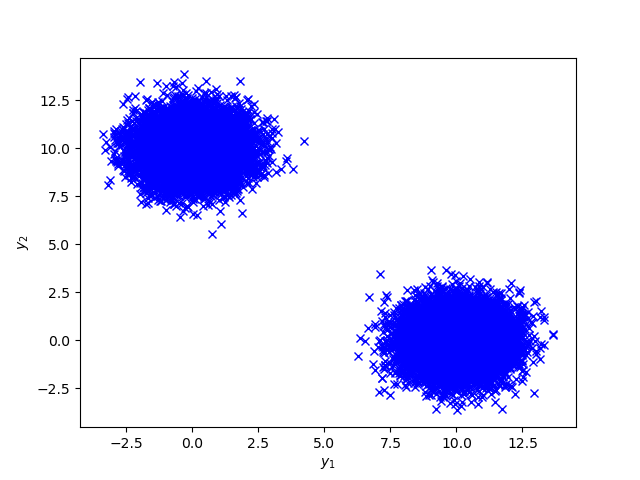
\includegraphics[width=\columnwidth]{./figs/twoD/scatter_plot.png}
\caption{Scatter plot of $\mbf{y} = \begin{pmatrix} y_1 \\ y_2 \end{pmatrix}$ for $A = 10$}
\label{fig:scatter_plt_y}
\end{figure}
%
\item
For the above problem, find a decision rule for detecting the symbols $\mbf{s}_0 $ and $\mbf{s}_1$.
\\
\solution The decision rule is
\begin{equation}
\label{eq:decision_rule}
y_1 \dec{s_0}{s_1} y_2
\end{equation}
%
\item
Plot 
\begin{equation} 
P_e = \pr{\hat{\mbf{x}} = \mbf{s}_1|\mbf{x} = \mbf{s}_0}
\end{equation}
with respect to the SNR from 0 to 10 dB.
\\
\begin{figure}
\centering
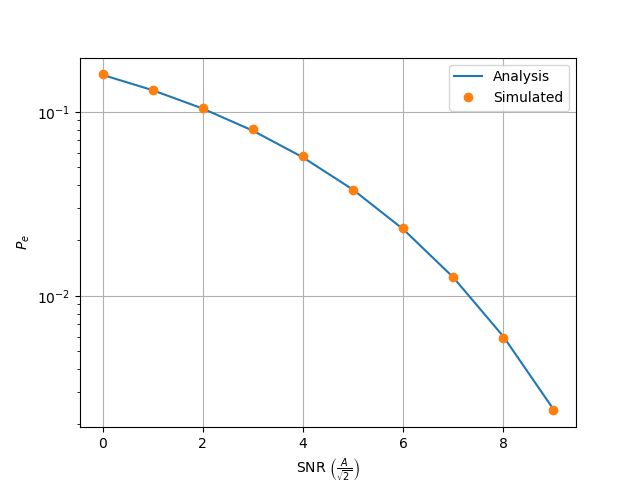
\includegraphics[width=\columnwidth]{./figs/twoD/ber_snr_plot.png}
\caption{$P_e$ with respect to SNR from 0 to 10 dB}
\label{fig:ber_snr_plot}
\end{figure}
%
\item
Obtain an expression for $P_e$. Verify this by comparing the theory and simulation plots on the same graph.
\\
\solution 
\begin{align}
P_e = \pr{\hat{\mbf{x}} = \mbf{s}_1|\mbf{x} = \mbf{s}_0}
\end{align}
Given that $\mbf{s}_0$ was transmitted, the received signal is
\begin{align}
\mbf{y}|\mbf{s}_0 = \begin{pmatrix} A \\ 0 \end{pmatrix} + \begin{pmatrix} n_1 \\ n_2 \end{pmatrix}
\end{align}
From \ref{eq:decision_rule}, the probability of error is given by 
\begin{align}
P_e &= \pr{y_1 < y_2 |\mbf{s}_0} = \pr{A+n_1 < n_2}\\
&= \pr{n_2 - n_1 > A}
\end{align}
Note that $n_2 - n_1 \sim \gauss{0}{2}$. Thus,
\begin{align}
P_e &= \pr{\sqrt{2}w > A}\\
\pr{w > \dfrac{A}{\sqrt{2}}}\\
\Rightarrow P_e &= \qfunc{\frac{A}{\sqrt{2}}}
\end{align}
where $w \sim \gauss{0}{1}$.
\end{enumerate}

%%
\section{Transform Domain: Moment Generating Function}
Let $X \sim \gauss{\mu}{\sigma^2}$.

\begin{enumerate}[label=\thesection.\arabic*.,ref=\thesection.\theenumi]
\numberwithin{equation}{enumi}
\numberwithin{figure}{enumi}
%%
\item
Find $M_{X}\brak{s} = E\sbrak{e^{-sX}}$.
\\
\solution The MGF of $X$ is
%
\begin{align}
M_{X}(s) &=\int_{-\infty}^{\infty}e^{-s X}p_{X}(x) dx 
\\
&=e^{-s\mu}e^{-\frac{s^2\sigma^2}{2}}
\label{eq:probman_mgf_X}
\end{align}
%
\item
Let 
%
\begin{equation}
N = n_1 - n_2, \quad   n_1,n_2 \sim \gauss{0}{1}.
\end{equation}
%
Find $M_{N}(s)$, assuming that $n_1$ and $n_2$ are independent.
\\
\solution Substituting from \eqref{eq:probman_mgf_X} and using independence,
\begin{align}
M_N(s)&=E[e^{-(n_1-n_2)s}]=M_{n_1}(s) M_{n_2}(-s)
\\
&= e^{-s^2\sigma^2} = e^{-s^2} \quad \brak{\because \sigma = 1}
\label{eq:probman_mgf_N}
\end{align}
%
\item
Show that $N$ is Gaussian. Find its mean and variance.  Comment.
\\
\solution From \eqref{eq:probman_mgf_N} and \eqref{eq:probman_mgf_X}, it is obvious that $X \sim \gauss{0}{2}$.  Thus,
%
the difference of two Gaussian random variables is also a Gaussian random variable.

\end{enumerate}

%%
\section{Uniform to Other: Quantile function}
\begin{enumerate}[label=\thesection.\arabic*.,ref=\thesection.\theenumi]
\numberwithin{equation}{enumi}
\numberwithin{figure}{enumi}
%%
%
%
\item
Generate samples of 
%
\begin{equation}
V = -2\ln\brak{1-U}
\label{eq:probman_V_cdf_sim}
\end{equation}
%
and plot its CDF.  Comment.
\\
\solution
Consider orthogonal vectors $\vec{m_1}$ and $\vec{m_2}$ to the given normal vector $\vec{n}$. Let, $\vec{m}$ = $\myvec{a\\b\\c}$, then
\begin{align}
\vec{m^T}\vec{n} &= 0\\
\implies\myvec{a&b&c}\myvec{3\\2\\-6} &= 0\\
\implies3a+2b-6c &= 0
\end{align}
Let a=1 and b=0 we get,
\begin{align}
\vec{m_1} &= \myvec{1\\0\\\frac{1}{2}} \label{eq:solutions/4/45/1/eq:eq1}
\end{align}
Let a=0 and b=1 we get,
\begin{align}
\vec{m_2} &= \myvec{0\\1\\\frac{1}{3}} \label{eq:solutions/4/45/1/eq:eq2}
\end{align}
Solving the equation,
\begin{align}
\vec{M}\vec{x} &= \vec{b}\label{eq:solutions/4/45/1/eq:eq3}
\end{align}
Substituting \eqref{eq:solutions/4/45/1/eq:eq1} and \eqref{eq:solutions/4/45/1/eq:eq2} in \eqref{eq:solutions/4/45/1/eq:eq3},
\begin{align}
    \myvec{1&0\\0&1\\\frac{1}{2}&\frac{1}{3}}\vec{x} &= \myvec{-3\\2\\1}\label{eq:solutions/4/45/1/eq:eq4}
\end{align}
Solving \eqref{eq:solutions/4/45/1/eq:eq4} using Singular Value Decomposition on $\vec{M}$ as follows,
\begin{align}
\vec{M}=\vec{U}\vec{\Sigma}\vec{V}^T\label{eq:solutions/4/45/1/eq:eq5}
\end{align}
Where the columns of $\vec{V}$ are the eigen vectors of $\vec{M}^T\vec{M}$ ,the columns of $\vec{U}$ are the eigen vectors of $\vec{M}\vec{M}^T$ and $\vec{S}$ is diagonal matrix of singular value of eigenvalues of $\vec{M}^T\vec{M}$. We have,
\begin{align}
\vec{M}^T\vec{M}=\myvec{\frac{5}{4}&\frac{1}{6}\\\frac{1}{6}&\frac{10}{9}}\label{eq:solutions/4/45/1/eq:eq6}\\
\vec{M}\vec{M}^T=\myvec{1&0&\frac{1}{2}\\0&1&\frac{1}{3}\\\frac{1}{2}&\frac{1}{3}&\frac{13}{36}}
\end{align}
Substituting \eqref{eq:solutions/4/45/1/eq:eq5} in \eqref{eq:solutions/4/45/1/eq:eq3},
\begin{align}
\vec{U}\vec{\Sigma}\vec{V}^T\vec{x} & = \vec{b}\\
\implies\vec{x} &= \vec{V}\vec{\Sigma^{-1}}\vec{U^T}\vec{b}\label{eq:solutions/4/45/1/eq:eq7}
\end{align}
Where $\vec{\Sigma^{-1}}$ is Moore-Penrose Pseudo-Inverse of $\vec{\Sigma}$ and is obtained by inversing only non-zero elements in $\vec{\Sigma}$\\
Calculating eigen values of $\vec{M}\vec{M}^T$,
\begin{align}
\mydet{\vec{M}\vec{M}^T - \lambda\vec{I}} &= 0\\
\implies\mydet{1-\lambda&0&\frac{1}{2}\\0&1-\lambda&\frac{1}{3}\\\frac{1}{2}&\frac{1}{3}&\frac{13}{36}-\lambda} &=0\\
\implies \lambda^3-\frac{85}{36}\lambda^2+\frac{49}{36}\lambda&=0 \label{eq:solutions/4/45/1/eq:eq8}
\end{align}
From the characteristic equation \eqref{eq:solutions/4/45/1/eq:eq8}, the eigen values of $\vec{M}\vec{M}^T$ are,
\begin{align}
\lambda_1 = \frac{49}{36} \quad
\lambda_2 = 1 \quad
\lambda_3 = 0
\end{align}
The eigen vectors of $\vec{M}\vec{M}^T$ are,
\begin{align}
\vec{u_1}=\myvec{\frac{18}{13}\\\frac{12}{13}\\1}\quad
\vec{u_2}=\myvec{\frac{-2}{3}\\1\\0}\quad
\vec{u_3}=\myvec{\frac{-1}{2}\\\frac{-1}{3}\\1}\label{eq:solutions/4/45/1/eq:eq9}
\end{align}
Normalizing the eigen vectors in equation \eqref{eq:solutions/4/45/1/eq:eq9}
\begin{align}
\vec{u_1}=\myvec{\frac{18}{7\sqrt{13}}\\\frac{12}{7\sqrt{13}}\\\frac{\sqrt{13}}{7}}\quad
\vec{u_2}=\myvec{\frac{-2}{\sqrt{13}}\\\frac{3}{\sqrt{13}}\\0}\quad
\vec{u_3}=\myvec{\frac{-7}{12}\\\frac{-7}{18}\\\frac{7}{6}}
\end{align}
Hence we obtain $\vec{U}$ as follows,
\begin{align}
\vec{U}=\myvec{\frac{18}{7\sqrt{13}}&\frac{-2}{\sqrt{13}}&\frac{-7}{12}\\\frac{12}{7\sqrt{13}}&\frac{3}{\sqrt{13}}&\frac{-7}{18}\\\frac{\sqrt{13}}{7}&0&\frac{7}{6}}\label{eq:solutions/4/45/1/eq:eq10}
\end{align}
By computing the singular values from eigen values $\lambda_1, \lambda_2, \lambda_3$ we get $\vec{\Sigma}$ as,
\begin{align}
\vec{\Sigma}=\myvec{\frac{49}{36}&0\\0&1\\0&0}
\end{align}
Calculating eigen values of $\vec{M}^T\vec{M}$,
\begin{align}
\mydet{\vec{M}^T\vec{M} - \lambda\vec{I}} &= 0\\
\implies\mydet{\frac{5}{4}-\lambda&\frac{1}{6}\\\frac{1}{6}&\frac{10}{9}-\lambda} &=0\\
\implies\lambda^2-\frac{85}{36}\lambda+\frac{49}{36} &=0
\end{align}
From the characteristic equation, the eigen values of $\vec{M}^T\vec{M}$ are,
\begin{align}
\lambda_1 = \frac{49}{36}\quad
\lambda_2 = 1
\end{align}
Hence the eigen vectors of $\vec{M}^T\vec{M}$ are,
\begin{align}
\vec{v}_1=\myvec{\frac{3}{2}\\1} \quad
\vec{v}_2=\myvec{\frac{-2}{3}\\1}
\end{align}
Normalizing the eigen vectors,
\begin{align}
\vec{v}_1=\myvec{\frac{3}{\sqrt{13}}\\\frac{2}{\sqrt{13}}} \quad
\vec{v}_2=\myvec{\frac{-2}{\sqrt{13}}\\\frac{3}{\sqrt{13}}}
\end{align}
Hence we obtain $\vec{V}$ as,
\begin{align}
\vec{V}=\myvec{\frac{3}{\sqrt{13}}&\frac{-2}{\sqrt{13}}\\\frac{2}{\sqrt{13}}&\frac{3}{\sqrt{13}}}
\end{align}
From \eqref{eq:solutions/4/45/1/eq:eq3}, the Singular Value Decomposition of $\vec{M}$ is as follows,
\begin{align}
\vec{M} = \myvec{\frac{18}{7\sqrt{13}}&\frac{-2}{\sqrt{13}}&\frac{-7}{12}\\\frac{12}{7\sqrt{13}}&\frac{3}{\sqrt{13}}&\frac{-7}{18}\\\frac{\sqrt{13}}{7}&0&\frac{7}{6}}\myvec{\frac{49}{36}&0\\0&1\\0&0}\myvec{\frac{3}{\sqrt{13}}&\frac{-2}{\sqrt{13}}\\\frac{2}{\sqrt{13}}&\frac{3}{\sqrt{13}}}^T
\end{align}
And, the Moore-Penrose Pseudo inverse of $\vec{\Sigma}$ is given by,
\begin{align}
\vec{\Sigma^{-1}} = \myvec{\frac{6}{7}&0&0\\0&1&0}
\end{align}
From \eqref{eq:solutions/4/45/1/eq:eq7} we get,
\begin{align}
\vec{U}^T\vec{b}&=\myvec{\frac{-17}{7\sqrt{13}}\\\frac{12}{\sqrt{13}}\\\frac{77}{36}}\\
\vec{\Sigma^{-1}}\vec{U}^T\vec{b}&=\myvec{\frac{-102}{49\sqrt{13}}\\\frac{12}{\sqrt{13}}}\\
\vec{x} &= \vec{V}\vec{\Sigma^{-1}}\vec{U}^T\vec{b} &= \myvec{\frac{-114}{49}\\\frac{120}{49}}\label{eq:solutions/4/45/1/eq:eq11}
\end{align}
Now we verify the solution \eqref{eq:solutions/4/45/1/eq:eq11} using,
\begin{align}
\vec{M}\vec{x}=\vec{b}
\implies\vec{M}^T\vec{M}\vec{x} = \vec{M}^T\vec{b}\label{eq:solutions/4/45/1/eqVerify}
\end{align}
On evaluating the R.H.S in \eqref{eq:solutions/4/45/1/eqVerify} we get,
\begin{align}
\vec{M}^T\vec{M}\vec{x} &= \myvec{\frac{-5}{2}\\\frac{7}{3}}\\
\implies\myvec{\frac{5}{4}&\frac{1}{6}\\\frac{1}{6}&\frac{10}{9}}\vec{x} &= \myvec{\frac{-5}{2}\\\frac{7}{3}}\label{eq:solutions/4/45/1/eq:eq12}
\end{align}
On solving the augmented matrix of \eqref{eq:solutions/4/45/1/eq:eq12} we get,
\begin{align}
\myvec{\frac{5}{4}&\frac{1}{6}&\frac{-5}{2}\\\frac{1}{6}&\frac{10}{9}&\frac{7}{3}} &\xleftrightarrow{R_1=\frac{4R_1}{5}}\myvec{1&\frac{2}{15}&-2\\\frac{1}{6}&\frac{10}{9}&\frac{7}{3}}\\
&\xleftrightarrow{R_2=R_2-\frac{R_1}{6}}\myvec{1&\frac{2}{15}&-2\\0&\frac{49}{45}&\frac{8}{3}}\\
&\xleftrightarrow{R_2=\frac{45}{49}R_2}\myvec{1&\frac{2}{15}&-2\\0&1&\frac{120}{49}}\\
&\xleftrightarrow{R_1=R_1-\frac{2R_2}{15}}\myvec{1&0&\frac{-114}{49}\\0&1&\frac{120}{49}}\label{eq:solutions/4/45/1/eq:eq13}
\end{align}
From equation \eqref{eq:solutions/4/45/1/eq:eq13}, solution is given by,
\begin{align}
\vec{x}=\myvec{\frac{-114}{49}\\\frac{120}{49}}\label{eq:solutions/4/45/1/eq:eq14}
\end{align}
From the equations \eqref{eq:solutions/4/45/1/eq:eq11} and \eqref{eq:solutions/4/45/1/eq:eq14}, the solution $\vec{x}$ is verified.


%
\item
Generate the Rayleigh distribution from Uniform. Verify your result through graphical plots.

\end{enumerate}

\section{Miscellaneous Distributions}
\begin{enumerate}[label=\thesection.\arabic*.,ref=\thesection.\theenumi]
\numberwithin{equation}{enumi}
\numberwithin{figure}{enumi}

\item A carton consists of 100 shirts of which 88 are good, 8 have minor defects and 4 have major defects.Jimmy, a trader, will only accept the shirts which are good, but Sujatha, another trader, will only reject the shirts which have major defects.One shirt is drawn at random from the carton. What is the probability that\\
(i) it is acceptable to Jimmy?\\
(ii) it is acceptable to Sujatha?
\\
\solution
From the given information, Table \ref{table:5.19} can be generated.
\begin{table}[!ht]
\centering
\resizebox{\columnwidth}{!}{
\begin{tabular}{|p{4cm}|p{4cm}|}
\hline
\multicolumn{2}{|c|}{\textbf{A Random variable which has 3 possible values}}\\ \hline
\multirow{2}{*}{$\pr{X=0}=\frac{4}{100}=0.04$} & out of 100, 4 have major defects shirts
\\
\hline
\multirow{2}{*}{$\pr{X=1}=\frac{8}{100}=0.08$} & out of 100,8 are accepted minor defected shirts\\ \hline
\multirow{2}{*}{$\pr{X=2}=\frac{88}{100}=0.88$} & out of 100,88 are accepted good shirts\\ \hline
\end{tabular}
}
\caption{Random variables}
\label{table:5.19}
\end{table}
Then
\begin{enumerate}
\item The probability that the shirt is acceptable to Jimmy is
\begin{align}
\pr{X=2}=\frac{88}{100}
\end{align}
%
\item The probability that the shirt is acceptable to Sujatha is
\begin{align}
1-\pr{X=0}=1-\frac{4}{100} = \frac{96}{100}
\end{align}

\end{enumerate}
%
The following code simulates the probability
\begin{lstlisting}
codes/misc/discrete.ipynb
\end{lstlisting}
\end{enumerate} 

%\section{Sum of i.i.d random variables}
%\input{./chapters/conv.tex}


\end{document}


